\PassOptionsToPackage{unicode=true}{hyperref} % options for packages loaded elsewhere
\PassOptionsToPackage{hyphens}{url}
\PassOptionsToPackage{dvipsnames,svgnames*,x11names*}{xcolor}
%
\documentclass[12pt, krantz2,]{krantz}
\usepackage{lmodern}
\usepackage{amssymb,amsmath}
\usepackage{ifxetex,ifluatex}
\usepackage{fixltx2e} % provides \textsubscript
\ifnum 0\ifxetex 1\fi\ifluatex 1\fi=0 % if pdftex
  \usepackage[T1]{fontenc}
  \usepackage[utf8]{inputenc}
  \usepackage{textcomp} % provides euro and other symbols
\else % if luatex or xelatex
  \usepackage{unicode-math}
  \defaultfontfeatures{Ligatures=TeX,Scale=MatchLowercase}
    \setmonofont[Mapping=tex-ansi,Scale=0.7]{Source Code Pro}
\fi
% use upquote if available, for straight quotes in verbatim environments
\IfFileExists{upquote.sty}{\usepackage{upquote}}{}
% use microtype if available
\IfFileExists{microtype.sty}{%
\usepackage[]{microtype}
\UseMicrotypeSet[protrusion]{basicmath} % disable protrusion for tt fonts
}{}
\IfFileExists{parskip.sty}{%
\usepackage{parskip}
}{% else
\setlength{\parindent}{0pt}
\setlength{\parskip}{6pt plus 2pt minus 1pt}
}
\usepackage{xcolor}
\usepackage{hyperref}
\hypersetup{
            pdftitle={HR Analytics in R},
            pdfauthor={Hendrik Feddersen},
            colorlinks=true,
            linkcolor=Maroon,
            filecolor=Maroon,
            citecolor=Blue,
            urlcolor=Blue,
            breaklinks=true}
\urlstyle{same}  % don't use monospace font for urls
\usepackage{color}
\usepackage{fancyvrb}
\newcommand{\VerbBar}{|}
\newcommand{\VERB}{\Verb[commandchars=\\\{\}]}
\DefineVerbatimEnvironment{Highlighting}{Verbatim}{commandchars=\\\{\}}
% Add ',fontsize=\small' for more characters per line
\usepackage{framed}
\definecolor{shadecolor}{RGB}{248,248,248}
\newenvironment{Shaded}{\begin{snugshade}}{\end{snugshade}}
\newcommand{\AlertTok}[1]{\textcolor[rgb]{0.33,0.33,0.33}{#1}}
\newcommand{\AnnotationTok}[1]{\textcolor[rgb]{0.37,0.37,0.37}{\textbf{\textit{#1}}}}
\newcommand{\AttributeTok}[1]{\textcolor[rgb]{0.61,0.61,0.61}{#1}}
\newcommand{\BaseNTok}[1]{\textcolor[rgb]{0.06,0.06,0.06}{#1}}
\newcommand{\BuiltInTok}[1]{#1}
\newcommand{\CharTok}[1]{\textcolor[rgb]{0.5,0.5,0.5}{#1}}
\newcommand{\CommentTok}[1]{\textcolor[rgb]{0.37,0.37,0.37}{\textit{#1}}}
\newcommand{\CommentVarTok}[1]{\textcolor[rgb]{0.37,0.37,0.37}{\textbf{\textit{#1}}}}
\newcommand{\ConstantTok}[1]{\textcolor[rgb]{0,0,0}{#1}}
\newcommand{\ControlFlowTok}[1]{\textcolor[rgb]{0.27,0.27,0.27}{\textbf{#1}}}
\newcommand{\DataTypeTok}[1]{\textcolor[rgb]{0.27,0.27,0.27}{#1}}
\newcommand{\DecValTok}[1]{\textcolor[rgb]{0.06,0.06,0.06}{#1}}
\newcommand{\DocumentationTok}[1]{\textcolor[rgb]{0.37,0.37,0.37}{\textbf{\textit{#1}}}}
\newcommand{\ErrorTok}[1]{\textcolor[rgb]{0.14,0.14,0.14}{\textbf{#1}}}
\newcommand{\ExtensionTok}[1]{#1}
\newcommand{\FloatTok}[1]{\textcolor[rgb]{0.06,0.06,0.06}{#1}}
\newcommand{\FunctionTok}[1]{\textcolor[rgb]{0,0,0}{#1}}
\newcommand{\ImportTok}[1]{#1}
\newcommand{\InformationTok}[1]{\textcolor[rgb]{0.37,0.37,0.37}{\textbf{\textit{#1}}}}
\newcommand{\KeywordTok}[1]{\textcolor[rgb]{0.27,0.27,0.27}{\textbf{#1}}}
\newcommand{\NormalTok}[1]{#1}
\newcommand{\OperatorTok}[1]{\textcolor[rgb]{0.43,0.43,0.43}{\textbf{#1}}}
\newcommand{\OtherTok}[1]{\textcolor[rgb]{0.37,0.37,0.37}{#1}}
\newcommand{\PreprocessorTok}[1]{\textcolor[rgb]{0.37,0.37,0.37}{\textit{#1}}}
\newcommand{\RegionMarkerTok}[1]{#1}
\newcommand{\SpecialCharTok}[1]{\textcolor[rgb]{0,0,0}{#1}}
\newcommand{\SpecialStringTok}[1]{\textcolor[rgb]{0.5,0.5,0.5}{#1}}
\newcommand{\StringTok}[1]{\textcolor[rgb]{0.5,0.5,0.5}{#1}}
\newcommand{\VariableTok}[1]{\textcolor[rgb]{0,0,0}{#1}}
\newcommand{\VerbatimStringTok}[1]{\textcolor[rgb]{0.5,0.5,0.5}{#1}}
\newcommand{\WarningTok}[1]{\textcolor[rgb]{0.37,0.37,0.37}{\textbf{\textit{#1}}}}
\usepackage{longtable,booktabs}
% Fix footnotes in tables (requires footnote package)
\IfFileExists{footnote.sty}{\usepackage{footnote}\makesavenoteenv{longtable}}{}
\usepackage{graphicx,grffile}
\makeatletter
\def\maxwidth{\ifdim\Gin@nat@width>\linewidth\linewidth\else\Gin@nat@width\fi}
\def\maxheight{\ifdim\Gin@nat@height>\textheight\textheight\else\Gin@nat@height\fi}
\makeatother
% Scale images if necessary, so that they will not overflow the page
% margins by default, and it is still possible to overwrite the defaults
% using explicit options in \includegraphics[width, height, ...]{}
\setkeys{Gin}{width=\maxwidth,height=\maxheight,keepaspectratio}
\setlength{\emergencystretch}{3em}  % prevent overfull lines
\providecommand{\tightlist}{%
  \setlength{\itemsep}{0pt}\setlength{\parskip}{0pt}}
\setcounter{secnumdepth}{5}
% Redefines (sub)paragraphs to behave more like sections
\ifx\paragraph\undefined\else
\let\oldparagraph\paragraph
\renewcommand{\paragraph}[1]{\oldparagraph{#1}\mbox{}}
\fi
\ifx\subparagraph\undefined\else
\let\oldsubparagraph\subparagraph
\renewcommand{\subparagraph}[1]{\oldsubparagraph{#1}\mbox{}}
\fi

% set default figure placement to htbp
\makeatletter
\def\fps@figure{htbp}
\makeatother

\usepackage{booktabs}
\usepackage{longtable}
\usepackage[bf,singlelinecheck=off]{caption}

\usepackage{framed,color}
\definecolor{shadecolor}{RGB}{248,248,248}

\usepackage{float}
\usepackage{array}
\usepackage{multirow}
%\usepackage[table]{xcolor}
\usepackage{wrapfig}
\usepackage{colortbl}
\usepackage{pdflscape}
\usepackage{tabu}
\usepackage{threeparttable}
\usepackage{threeparttablex}
\usepackage[normalem]{ulem}
\usepackage{makecell}

\renewcommand{\textfraction}{0.05}
\renewcommand{\topfraction}{0.8}
\renewcommand{\bottomfraction}{0.8}
\renewcommand{\floatpagefraction}{0.75}

\renewenvironment{quote}{\begin{VF}}{\end{VF}}
\let\oldhref\href
\renewcommand{\href}[2]{#2\footnote{\url{#1}}}

\makeatletter
\newenvironment{kframe}{%
\medskip{}
\setlength{\fboxsep}{.8em}
 \def\at@end@of@kframe{}%
 \ifinner\ifhmode%
  \def\at@end@of@kframe{\end{minipage}}%
  \begin{minipage}{\columnwidth}%
 \fi\fi%
 \def\FrameCommand##1{\hskip\@totalleftmargin \hskip-\fboxsep
 \colorbox{shadecolor}{##1}\hskip-\fboxsep
     % There is no \\@totalrightmargin, so:
     \hskip-\linewidth \hskip-\@totalleftmargin \hskip\columnwidth}%
 \MakeFramed {\advance\hsize-\width
   \@totalleftmargin\z@ \linewidth\hsize
   \@setminipage}}%
 {\par\unskip\endMakeFramed%
 \at@end@of@kframe}
\makeatother

\renewenvironment{Shaded}{\begin{kframe}}{\end{kframe}}

\usepackage{makeidx}
\makeindex

\urlstyle{tt}

%% Need to clean up
\newenvironment{rmdblock}[1]
  {\begin{shaded*}
  \begin{itemize}
  \renewcommand{\labelitemi}{
    \raisebox{-.7\height}[0pt][0pt]{
  %    {\setkeys{Gin}{width=3em,keepaspectratio}\includegraphics{images/#1}}
    }
  }
  \item
  }
  {
  \end{itemize}
  \end{shaded*}
  }

\newenvironment{rmdnote}
  {\begin{rmdblock}{note}}
  {\end{rmdblock}}
\newenvironment{rmdcaution}
  {\begin{rmdblock}{caution}}
  {\end{rmdblock}}
\newenvironment{rmdimportant}
  {\begin{rmdblock}{important}}
  {\end{rmdblock}}
\newenvironment{rmdtip}
  {\begin{rmdblock}{tip}}
  {\end{rmdblock}}
\newenvironment{rmdwarning}
  {\begin{rmdblock}{warning}}
  {\end{rmdblock}}
\newenvironment{learncheck}
  {\begin{rmdblock}{warning}}
  {\end{rmdblock}}
\newenvironment{review}
  {\begin{rmdblock}{warning}}
  {\end{rmdblock}}
\newenvironment{announcement}
  {\begin{rmdblock}{warning}}
  {\end{rmdblock}}


\usepackage{amsthm}
\makeatletter
\def\thm@space@setup{%
  \thm@preskip=8pt plus 2pt minus 4pt
  \thm@postskip=\thm@preskip
}
\makeatother

\frontmatter
\usepackage[]{natbib}
\bibliographystyle{apalike}

\title{HR Analytics in R}
\providecommand{\subtitle}[1]{}
\subtitle{Common tasks achieved with the power of R}
\author{Hendrik Feddersen}
\date{May 04, 2019}

\begin{document}
\maketitle

% you may need to leave a few empty pages before the dedication page

%\cleardoublepage\newpage\thispagestyle{empty}\null
%\cleardoublepage\newpage\thispagestyle{empty}\null
%\cleardoublepage\newpage
\thispagestyle{empty}

\begin{center}
%\includegraphics{images/dedication.pdf}
\end{center}

\setlength{\abovedisplayskip}{-5pt}
\setlength{\abovedisplayshortskip}{-5pt}

{
\hypersetup{linkcolor=}
\setcounter{tocdepth}{2}
\tableofcontents
}
\listoftables
\listoffigures
\hypertarget{intro}{%
\chapter{Introduction}\label{intro}}

Placeholder

\hypertarget{sec:intro-for-students}{%
\section{Introduction for students}\label{sec:intro-for-students}}

\hypertarget{workingwithmaterials}{%
\subsection*{Working with the material}\label{workingwithmaterials}}


\hypertarget{conventions}{%
\subsection*{Conventions}\label{conventions}}


\hypertarget{subsec:learning-goals}{%
\subsection{What you will learn from this book}\label{subsec:learning-goals}}

\hypertarget{subsec:pipeline}{%
\subsection{Data/science pipeline}\label{subsec:pipeline}}

\hypertarget{subsec:reproducible}{%
\subsection{Reproducible research}\label{subsec:reproducible}}

\hypertarget{final-note-for-students}{%
\subsection{Final note for students}\label{final-note-for-students}}

\hypertarget{sec:intro-instructors}{%
\section{Introduction for instructors}\label{sec:intro-instructors}}

\hypertarget{who-is-this-book-for}{%
\subsection{Who is this book for?}\label{who-is-this-book-for}}

\hypertarget{sec:connect-contribute}{%
\section{Connect and contribute}\label{sec:connect-contribute}}

\hypertarget{sec:about-book}{%
\section{About this book}\label{sec:about-book}}

\hypertarget{sec:about-authors}{%
\section{About the author}\label{sec:about-authors}}

\hypertarget{colophon}{%
\subsection{Colophon}\label{colophon}}

\hypertarget{getting-started}{%
\chapter{Getting Started with Data in R}\label{getting-started}}

Placeholder

\hypertarget{r-rstudio}{%
\section{What are R and RStudio?}\label{r-rstudio}}

\hypertarget{installing-r-and-rstudio}{%
\subsection{Installing R and RStudio}\label{installing-r-and-rstudio}}

\hypertarget{using-r-via-rstudio}{%
\subsection{Using R via RStudio}\label{using-r-via-rstudio}}

\hypertarget{code}{%
\section{How do I code in R?}\label{code}}

\hypertarget{programming-concepts}{%
\subsection{Basic programming concepts and terminology}\label{programming-concepts}}

\hypertarget{errors-warnings-and-messages}{%
\subsection{Errors, warnings, and messages}\label{errors-warnings-and-messages}}

\hypertarget{tips-on-learning-to-code}{%
\subsection{Tips on learning to code}\label{tips-on-learning-to-code}}

\hypertarget{packages}{%
\section{What are R packages?}\label{packages}}

\hypertarget{package-installation}{%
\subsection{Package installation}\label{package-installation}}

\hypertarget{package-loading}{%
\subsection{Package loading}\label{package-loading}}

\hypertarget{package-use}{%
\subsection{Package use}\label{package-use}}

\hypertarget{nycflights13}{%
\section{Explore your first datasets}\label{nycflights13}}

\hypertarget{nycflights13-package}{%
\subsection{\texorpdfstring{\texttt{nycflights13} package}{nycflights13 package}}\label{nycflights13-package}}

\hypertarget{flights-data-frame}{%
\subsection{\texorpdfstring{\texttt{flights} data frame}{flights data frame}}\label{flights-data-frame}}

\hypertarget{exploredataframes}{%
\subsection{Exploring data frames}\label{exploredataframes}}

\hypertarget{identification-vs-measurement-variables}{%
\subsection{Identification \& measurement variables}\label{identification-vs-measurement-variables}}

\hypertarget{help-files}{%
\subsection{Help files}\label{help-files}}

\hypertarget{conclusion}{%
\section{Conclusion}\label{conclusion}}

\hypertarget{additional-resources}{%
\subsection{Additional resources}\label{additional-resources}}

\hypertarget{whats-to-come}{%
\subsection{What's to come?}\label{whats-to-come}}

\hypertarget{part-data-science-via-the-tidyverse}{%
\part{Data Science via the tidyverse}\label{part-data-science-via-the-tidyverse}}

\hypertarget{viz}{%
\chapter{Data Visualization}\label{viz}}

Placeholder

\hypertarget{needed-packages}{%
\subsection*{Needed packages}\label{needed-packages}}


\hypertarget{grammarofgraphics}{%
\section{The Grammar of Graphics}\label{grammarofgraphics}}

\hypertarget{components-of-the-grammar}{%
\subsection{Components of the Grammar}\label{components-of-the-grammar}}

\hypertarget{gapminder}{%
\subsection{Gapminder data}\label{gapminder}}

\hypertarget{other-components}{%
\subsection{Other components}\label{other-components}}

\hypertarget{ggplot2-package}{%
\subsection{ggplot2 package}\label{ggplot2-package}}

\hypertarget{FiveNG}{%
\section{Five Named Graphs - The 5NG}\label{FiveNG}}

\hypertarget{scatterplots}{%
\section{5NG\#1: Scatterplots}\label{scatterplots}}

\hypertarget{geompoint}{%
\subsection{Scatterplots via geom\_point}\label{geompoint}}

\hypertarget{overplotting}{%
\subsection{Over-plotting}\label{overplotting}}

\hypertarget{summary}{%
\subsection{Summary}\label{summary}}

\hypertarget{linegraphs}{%
\section{5NG\#2: Linegraphs}\label{linegraphs}}

\hypertarget{geomline}{%
\subsection{Linegraphs via geom\_line}\label{geomline}}

\hypertarget{summary-1}{%
\subsection{Summary}\label{summary-1}}

\hypertarget{histograms}{%
\section{5NG\#3: Histograms}\label{histograms}}

\hypertarget{geomhistogram}{%
\subsection{Histograms via geom\_histogram}\label{geomhistogram}}

\hypertarget{adjustbins}{%
\subsection{Adjusting the bins}\label{adjustbins}}

\hypertarget{summary-2}{%
\subsection{Summary}\label{summary-2}}

\hypertarget{facets}{%
\section{Facets}\label{facets}}

\hypertarget{boxplots}{%
\section{5NG\#4: Boxplots}\label{boxplots}}

\hypertarget{geomboxplot}{%
\subsection{Boxplots via geom\_boxplot}\label{geomboxplot}}

\hypertarget{summary-3}{%
\subsection{Summary}\label{summary-3}}

\hypertarget{geombar}{%
\section{5NG\#5: Barplots}\label{geombar}}

\hypertarget{barplots-via-geom_bar-or-geom_col}{%
\subsection{Barplots via geom\_bar or geom\_col}\label{barplots-via-geom_bar-or-geom_col}}

\hypertarget{must-avoid-pie-charts}{%
\subsection{Must avoid pie charts!}\label{must-avoid-pie-charts}}

\hypertarget{two-categ-barplot}{%
\subsection{Two categorical variables}\label{two-categ-barplot}}

\hypertarget{summary-4}{%
\subsection{Summary}\label{summary-4}}

\hypertarget{conclusion-1}{%
\section{Conclusion}\label{conclusion-1}}

\hypertarget{summary-table}{%
\subsection{Summary table}\label{summary-table}}

\hypertarget{argument-specification}{%
\subsection{Argument specification}\label{argument-specification}}

\hypertarget{additional-resources-1}{%
\subsection{Additional resources}\label{additional-resources-1}}

\hypertarget{whats-to-come-3}{%
\subsection{What's to come}\label{whats-to-come-3}}

\hypertarget{wrangling}{%
\chapter{Data Wrangling}\label{wrangling}}

Placeholder

\hypertarget{needed-packages-1}{%
\subsection*{Needed packages}\label{needed-packages-1}}


\hypertarget{piping}{%
\section{\texorpdfstring{The pipe operator: \texttt{\%\textgreater{}\%}}{The pipe operator: \%\textgreater{}\%}}\label{piping}}

\hypertarget{filter}{%
\section{\texorpdfstring{\texttt{filter} rows}{filter rows}}\label{filter}}

\hypertarget{summarize}{%
\section{\texorpdfstring{\texttt{summarize} variables}{summarize variables}}\label{summarize}}

\hypertarget{groupby}{%
\section{\texorpdfstring{\texttt{group\_by} rows}{group\_by rows}}\label{groupby}}

\hypertarget{grouping-by-more-than-one-variable}{%
\subsection{Grouping by more than one variable}\label{grouping-by-more-than-one-variable}}

\hypertarget{mutate}{%
\section{\texorpdfstring{\texttt{mutate} existing variables}{mutate existing variables}}\label{mutate}}

\hypertarget{arrange}{%
\section{\texorpdfstring{\texttt{arrange} and sort rows}{arrange and sort rows}}\label{arrange}}

\hypertarget{joins}{%
\section{\texorpdfstring{\texttt{join} data frames}{join data frames}}\label{joins}}

\hypertarget{matching-key-variable-names}{%
\subsection{Matching ``key'' variable names}\label{matching-key-variable-names}}

\hypertarget{diff-key}{%
\subsection{Different ``key'' variable names}\label{diff-key}}

\hypertarget{multiple-key-variables}{%
\subsection{Multiple ``key'' variables}\label{multiple-key-variables}}

\hypertarget{normal-forms}{%
\subsection{Normal forms}\label{normal-forms}}

\hypertarget{other-verbs}{%
\section{Other verbs}\label{other-verbs}}

\hypertarget{select}{%
\subsection{\texorpdfstring{\texttt{select} variables}{select variables}}\label{select}}

\hypertarget{rename}{%
\subsection{\texorpdfstring{\texttt{rename} variables}{rename variables}}\label{rename}}

\hypertarget{top_n-values-of-a-variable}{%
\subsection{\texorpdfstring{\texttt{top\_n} values of a variable}{top\_n values of a variable}}\label{top_n-values-of-a-variable}}

\hypertarget{conclusion-2}{%
\section{Conclusion}\label{conclusion-2}}

\hypertarget{summary-table-1}{%
\subsection{Summary table}\label{summary-table-1}}

\hypertarget{additional-resources-2}{%
\subsection{Additional resources}\label{additional-resources-2}}

\hypertarget{whats-to-come-1}{%
\subsection{What's to come?}\label{whats-to-come-1}}

\hypertarget{tidy}{%
\chapter{Data Importing \& ``Tidy'' Data}\label{tidy}}

Placeholder

\hypertarget{needed-packages-2}{%
\subsection*{Needed packages}\label{needed-packages-2}}


\hypertarget{csv}{%
\section{Importing data}\label{csv}}

\hypertarget{using-the-console}{%
\subsection{Using the console}\label{using-the-console}}

\hypertarget{using-rstudios-interface}{%
\subsection{Using RStudio's interface}\label{using-rstudios-interface}}

\hypertarget{tidy-data-ex}{%
\section{Tidy data}\label{tidy-data-ex}}

\hypertarget{definition-of-tidy-data}{%
\subsection{Definition of ``tidy'' data}\label{definition-of-tidy-data}}

\hypertarget{converting-to-tidy-data}{%
\subsection{Converting to ``tidy'' data}\label{converting-to-tidy-data}}

\hypertarget{nycflights13-package-1}{%
\subsection{\texorpdfstring{\texttt{nycflights13} package}{nycflights13 package}}\label{nycflights13-package-1}}

\hypertarget{case-study-tidy}{%
\section{Case study: Democracy in Guatemala}\label{case-study-tidy}}

\hypertarget{conclusion-3}{%
\section{Conclusion}\label{conclusion-3}}

\hypertarget{tidyverse-package}{%
\subsection{\texorpdfstring{\texttt{tidyverse} package}{tidyverse package}}\label{tidyverse-package}}

\hypertarget{additional-resources-3}{%
\subsection{Additional resources}\label{additional-resources-3}}

\hypertarget{whats-to-come-2}{%
\subsection{What's to come?}\label{whats-to-come-2}}

\hypertarget{part-data-modeling-via-moderndive}{%
\part{Data Modeling via moderndive}\label{part-data-modeling-via-moderndive}}

\hypertarget{regression}{%
\chapter{Basic Regression}\label{regression}}

Placeholder

\hypertarget{needed-packages-3}{%
\subsection*{Needed packages}\label{needed-packages-3}}


\hypertarget{model1}{%
\section{One numerical explanatory variable}\label{model1}}

\hypertarget{model1EDA}{%
\subsection{Exploratory data analysis}\label{model1EDA}}

\hypertarget{model1table}{%
\subsection{Simple linear regression}\label{model1table}}

\hypertarget{model1points}{%
\subsection{Observed/fitted values and residuals}\label{model1points}}

\hypertarget{model2}{%
\section{One categorical explanatory variable}\label{model2}}

\hypertarget{model2EDA}{%
\subsection{Exploratory data analysis}\label{model2EDA}}

\hypertarget{model2table}{%
\subsection{Linear regression}\label{model2table}}

\hypertarget{model2points}{%
\subsection{Observed/fitted values and residuals}\label{model2points}}

\hypertarget{related-topics}{%
\section{Related topics}\label{related-topics}}

\hypertarget{correlation-is-not-causation}{%
\subsection{Correlation is not necessarily causation}\label{correlation-is-not-causation}}

\hypertarget{leastsquares}{%
\subsection{Best fitting line}\label{leastsquares}}

\hypertarget{underthehood}{%
\subsection{\texorpdfstring{\texttt{get\_regression\_x()} functions}{get\_regression\_x() functions}}\label{underthehood}}

\hypertarget{conclusion-4}{%
\section{Conclusion}\label{conclusion-4}}

\hypertarget{additional-resources-basic-regression}{%
\subsection{Additional resources}\label{additional-resources-basic-regression}}

\hypertarget{whats-to-come-4}{%
\subsection{What's to come?}\label{whats-to-come-4}}

\hypertarget{multiple-regression}{%
\chapter{Multiple Regression}\label{multiple-regression}}

Placeholder

\hypertarget{needed-packages-4}{%
\subsection*{Needed packages}\label{needed-packages-4}}


\hypertarget{model4}{%
\section{One numerical \& one categorical explanatory variable}\label{model4}}

\hypertarget{model4EDA}{%
\subsection{Exploratory data analysis}\label{model4EDA}}

\hypertarget{model4interactiontable}{%
\subsection{Interaction model}\label{model4interactiontable}}

\hypertarget{model4table}{%
\subsection{Parallel slopes model}\label{model4table}}

\hypertarget{model4points}{%
\subsection{Observed/fitted values and residuals}\label{model4points}}

\hypertarget{model3}{%
\section{Two numerical explanatory variables}\label{model3}}

\hypertarget{model3EDA}{%
\subsection{Exploratory data analysis}\label{model3EDA}}

\hypertarget{model3table}{%
\subsection{Regression plane}\label{model3table}}

\hypertarget{model3points}{%
\subsection{Observed/fitted values and residuals}\label{model3points}}

\hypertarget{related-topics-1}{%
\section{Related topics}\label{related-topics-1}}

\hypertarget{model-selection}{%
\subsection{Model selection}\label{model-selection}}

\hypertarget{correlationcoefficient2}{%
\subsection{Correlation coefficient}\label{correlationcoefficient2}}

\hypertarget{simpsonsparadox}{%
\subsection{Simpson's Paradox}\label{simpsonsparadox}}

\hypertarget{conclusion-5}{%
\section{Conclusion}\label{conclusion-5}}

\hypertarget{additional-resources-4}{%
\subsection{Additional resources}\label{additional-resources-4}}

\hypertarget{whats-to-come-5}{%
\subsection{What's to come?}\label{whats-to-come-5}}

\hypertarget{part-statistical-inference-via-infer}{%
\part{Statistical inference via infer}\label{part-statistical-inference-via-infer}}

\hypertarget{sampling}{%
\chapter{Sampling}\label{sampling}}

Placeholder

\hypertarget{needed-packages-5}{%
\subsection*{Needed packages}\label{needed-packages-5}}


\hypertarget{sampling-activity}{%
\section{Sampling activity}\label{sampling-activity}}

\hypertarget{what-proportion-of-this-bowls-balls-are-red}{%
\subsection{What proportion of this bowl's balls are red?}\label{what-proportion-of-this-bowls-balls-are-red}}

\hypertarget{using-the-shovel-once}{%
\subsection{Using the shovel once}\label{using-the-shovel-once}}

\hypertarget{student-shovels}{%
\subsection{Using the shovel 33 times}\label{student-shovels}}

\hypertarget{what-are-we-doing-here}{%
\subsection{What are we doing here?}\label{what-are-we-doing-here}}

\hypertarget{sampling-simulation}{%
\section{Computer simulation of sampling}\label{sampling-simulation}}

\hypertarget{using-the-virtual-shovel-once}{%
\subsection{Using the virtual shovel once}\label{using-the-virtual-shovel-once}}

\hypertarget{using-the-virtual-shovel-33-times}{%
\subsection{Using the virtual shovel 33 times}\label{using-the-virtual-shovel-33-times}}

\hypertarget{shovel-1000-times}{%
\subsection{Using the virtual shovel 1000 times}\label{shovel-1000-times}}

\hypertarget{different-shovels}{%
\subsection{Using different shovels}\label{different-shovels}}

\hypertarget{sampling-framework}{%
\section{Sampling framework}\label{sampling-framework}}

\hypertarget{terminology-and-notation}{%
\subsection{Terminology \& notation}\label{terminology-and-notation}}

\hypertarget{statistical-definitions}{%
\subsection{Statistical definitions}\label{statistical-definitions}}

\hypertarget{the-moral-of-the-story}{%
\subsection{The moral of the story}\label{the-moral-of-the-story}}

\hypertarget{sampling-case-study}{%
\section{Case study: Polls}\label{sampling-case-study}}

\hypertarget{sampling-conclusion}{%
\section{Conclusion}\label{sampling-conclusion}}

\hypertarget{sampling-conclusion-sampling-vs-assignment}{%
\subsection{Random sampling vs random assignment}\label{sampling-conclusion-sampling-vs-assignment}}

\hypertarget{sampling-conclusion-central-limit-theorem}{%
\subsection{Central Limit Theorem}\label{sampling-conclusion-central-limit-theorem}}

\hypertarget{sampling-conclusion-table}{%
\subsection{Summary table}\label{sampling-conclusion-table}}

\hypertarget{additional-resources-5}{%
\subsection{Additional resources}\label{additional-resources-5}}

\hypertarget{whats-to-come-6}{%
\subsection{What's to come?}\label{whats-to-come-6}}

\hypertarget{confidence-intervals}{%
\chapter{Confidence Intervals}\label{confidence-intervals}}

Placeholder

\hypertarget{needed-packages-6}{%
\subsection*{Needed packages}\label{needed-packages-6}}


\hypertarget{resampling-activity}{%
\section{Resampling activity}\label{resampling-activity}}

\hypertarget{what-is-the-average-year-of-circulated-us-pennies-in-2019}{%
\subsection{What is the average year of circulated US pennies in 2019?}\label{what-is-the-average-year-of-circulated-us-pennies-in-2019}}

\hypertarget{exploratory-data-analysis-on-original-sample}{%
\subsubsection*{Exploratory data analysis on original sample}\label{exploratory-data-analysis-on-original-sample}}


\hypertarget{using-resampling-once}{%
\subsection{Using resampling once}\label{using-resampling-once}}

\hypertarget{exploratory-data-analysis-on-the-resample}{%
\subsubsection*{Exploratory data analysis on the resample}\label{exploratory-data-analysis-on-the-resample}}


\hypertarget{student-resamples}{%
\subsection{Using resampling 33 times}\label{student-resamples}}

\hypertarget{whats-the-plan}{%
\subsection{What's the plan?}\label{whats-the-plan}}

\hypertarget{resampling-simulation}{%
\section{Computer simulation of resampling}\label{resampling-simulation}}

\hypertarget{using-the-virtual-resample-once}{%
\subsection{Using the virtual resample once}\label{using-the-virtual-resample-once}}

\hypertarget{using-the-virtual-resample-33-times}{%
\subsection{Using the virtual resample 33 times}\label{using-the-virtual-resample-33-times}}

\hypertarget{using-the-virtual-resample-1000-times}{%
\subsection{Using the virtual resample 1000 times}\label{using-the-virtual-resample-1000-times}}

\hypertarget{ci-build-up}{%
\section{Confidence interval build-up}\label{ci-build-up}}

\hypertarget{percentile-method}{%
\subsection{The percentile method}\label{percentile-method}}

\hypertarget{the-standard-error-method}{%
\subsection{The standard error method}\label{the-standard-error-method}}

\hypertarget{bootstrap-process}{%
\section{The bootstrapping framework}\label{bootstrap-process}}

\hypertarget{the-original-workflow-needed-for-this}{%
\subsection{The original workflow needed for this}\label{the-original-workflow-needed-for-this}}

\hypertarget{the-infer-package-for-statistical-inference}{%
\subsection{The infer package for statistical inference}\label{the-infer-package-for-statistical-inference}}

\hypertarget{specify-variables}{%
\subsubsection*{Specify variables}\label{specify-variables}}


\hypertarget{generate-replicates}{%
\subsubsection*{Generate replicates}\label{generate-replicates}}


\hypertarget{calculate-summary-statistics}{%
\subsubsection*{Calculate summary statistics}\label{calculate-summary-statistics}}


\hypertarget{observed-statistic-point-estimate-calculations}{%
\subsubsection*{Observed statistic / point estimate calculations}\label{observed-statistic-point-estimate-calculations}}


\hypertarget{visualize-the-results}{%
\subsubsection*{Visualize the results}\label{visualize-the-results}}


\hypertarget{infer-ci}{%
\subsection{Building confidence intervals with the infer package}\label{infer-ci}}

\hypertarget{percentile-method-infer}{%
\subsection{The percentile method with infer}\label{percentile-method-infer}}

\hypertarget{the-standard-error-method-with-infer}{%
\subsection{The standard error method with infer}\label{the-standard-error-method-with-infer}}

\hypertarget{one-prop-ci}{%
\section{Case study: Revisiting the red ball example}\label{one-prop-ci}}

\hypertarget{observed-statistic}{%
\subsection{Observed statistic}\label{observed-statistic}}

\hypertarget{one-prop-boot}{%
\subsection{Bootstrap distribution for one proportion}\label{one-prop-boot}}

\hypertarget{interpreting-the-confidence-interval}{%
\section{Interpreting the confidence interval}\label{interpreting-the-confidence-interval}}

\hypertarget{back-to-our-pennies-example}{%
\subsubsection*{Back to our pennies example}\label{back-to-our-pennies-example}}


\hypertarget{the-width-of-confidence-intervals}{%
\subsection*{The width of confidence intervals}\label{the-width-of-confidence-intervals}}


\hypertarget{the-impact-of-confidence-levels}{%
\subsubsection*{The impact of confidence levels}\label{the-impact-of-confidence-levels}}


\hypertarget{the-impact-of-sample-size}{%
\subsubsection*{The impact of sample size}\label{the-impact-of-sample-size}}


\hypertarget{case-study-two-prop-ci}{%
\section{Case study: Comparing two proportions}\label{case-study-two-prop-ci}}

\hypertarget{compute-the-point-estimate}{%
\subsection{Compute the point estimate}\label{compute-the-point-estimate}}

\hypertarget{bootstrap-distribution}{%
\subsection{Bootstrap distribution}\label{bootstrap-distribution}}

\hypertarget{ci-conclusion}{%
\section{Conclusion}\label{ci-conclusion}}

\hypertarget{comparing-bootstrap-and-sampling-distributions}{%
\subsection{Comparing bootstrap and sampling distributions}\label{comparing-bootstrap-and-sampling-distributions}}

\hypertarget{sampling-distribution}{%
\subsubsection*{Sampling distribution}\label{sampling-distribution}}


\hypertarget{bootstrap-distribution-1}{%
\subsubsection*{Bootstrap distribution}\label{bootstrap-distribution-1}}


\hypertarget{theory-ci}{%
\subsection{Theory-based confidence intervals}\label{theory-ci}}

\hypertarget{procedure-for-building-a-theory-based-ci-for-p}{%
\subsubsection*{\texorpdfstring{Procedure for building a theory-based CI for \(p\)}{Procedure for building a theory-based CI for p}}\label{procedure-for-building-a-theory-based-ci-for-p}}


\hypertarget{confidence-intervals-based-on-33-tactile-samples}{%
\subsubsection*{Confidence intervals based on 33 tactile samples}\label{confidence-intervals-based-on-33-tactile-samples}}


\hypertarget{confidence-intervals-based-on-100-virtual-samples}{%
\subsubsection*{Confidence intervals based on 100 virtual samples}\label{confidence-intervals-based-on-100-virtual-samples}}


\hypertarget{where-does-the-1.96-come-from}{%
\subsubsection*{Where does the 1.96 come from?}\label{where-does-the-1.96-come-from}}


\hypertarget{ci-conclusion-table}{%
\subsection{Summary table}\label{ci-conclusion-table}}

\hypertarget{additional-resources-6}{%
\subsection{Additional resources}\label{additional-resources-6}}

\hypertarget{whats-to-come-7}{%
\subsection{What's to come?}\label{whats-to-come-7}}

\hypertarget{hypothesis-testing}{%
\chapter{Hypothesis Testing}\label{hypothesis-testing}}

Placeholder

\hypertarget{needed-packages-7}{%
\subsection*{Needed packages}\label{needed-packages-7}}


\hypertarget{ht-activity}{%
\section{Hypothesis testing activity}\label{ht-activity}}

\hypertarget{question-of-interest}{%
\subsection{Question of interest}\label{question-of-interest}}

\hypertarget{what-did-we-actually-observe}{%
\subsection{What did we actually observe?}\label{what-did-we-actually-observe}}

\hypertarget{using-permuting-once}{%
\subsection{Using permuting once}\label{using-permuting-once}}

\hypertarget{using-permuting-33-times}{%
\subsection{Using permuting 33 times}\label{using-permuting-33-times}}

\hypertarget{ht-infer}{%
\section{Hypothesis testing with infer}\label{ht-infer}}

\hypertarget{revisiting-the-infer-verb-framework}{%
\subsection{Revisiting the infer verb framework}\label{revisiting-the-infer-verb-framework}}

\hypertarget{the-infer-pipeline-for-the-activity}{%
\subsection{\texorpdfstring{The \texttt{infer} pipeline for the activity}{The infer pipeline for the activity}}\label{the-infer-pipeline-for-the-activity}}

\hypertarget{choose-the-variables-of-interest}{%
\subsubsection*{Choose the variables of interest}\label{choose-the-variables-of-interest}}


\hypertarget{set-the-model-for-the-null-hypothesis}{%
\subsubsection*{Set the model for the null hypothesis}\label{set-the-model-for-the-null-hypothesis}}


\hypertarget{replicate-samples-assuming-the-null-hypothesis-is-true}{%
\subsubsection*{Replicate samples assuming the null hypothesis is true}\label{replicate-samples-assuming-the-null-hypothesis-is-true}}


\hypertarget{compute-the-statistic-for-each-replicate}{%
\subsubsection*{Compute the statistic for each replicate}\label{compute-the-statistic-for-each-replicate}}


\hypertarget{only-one-test}{%
\subsection{The ``There Is Only One Test'' framework}\label{only-one-test}}

\hypertarget{p-value}{%
\section{The p-value}\label{p-value}}

\hypertarget{corresponding-confidence-interval}{%
\subsection{Corresponding confidence interval}\label{corresponding-confidence-interval}}

\hypertarget{summary-5}{%
\subsection{Summary}\label{summary-5}}

\hypertarget{ht-interpretation}{%
\section{Interpretation of hypothesis testing results}\label{ht-interpretation}}

\hypertarget{trial}{%
\subsection{Criminal trial analogy}\label{trial}}

\hypertarget{two-possible-conclusions}{%
\subsubsection*{Two possible conclusions}\label{two-possible-conclusions}}


\hypertarget{types-of-errors-in-hypothesis-testing}{%
\subsection{Types of errors in hypothesis testing}\label{types-of-errors-in-hypothesis-testing}}

\hypertarget{logic-of-hypothesis-testing}{%
\subsubsection*{Logic of hypothesis testing}\label{logic-of-hypothesis-testing}}


\hypertarget{statistical-significance}{%
\subsection{Statistical significance}\label{statistical-significance}}

\hypertarget{ht-case-study}{%
\section{Case study: comparing two means}\label{ht-case-study}}

\hypertarget{randomizationpermutation}{%
\subsection{Randomization/permutation}\label{randomizationpermutation}}

\hypertarget{comparing-action-and-romance-movies}{%
\subsection{Comparing action and romance movies}\label{comparing-action-and-romance-movies}}

\hypertarget{sampling-rightarrow-randomization}{%
\subsection{\texorpdfstring{Sampling \(\rightarrow\) randomization}{Sampling \textbackslash{}rightarrow randomization}}\label{sampling-rightarrow-randomization}}

\hypertarget{data}{%
\subsection{Data}\label{data}}

\hypertarget{model-of-h_0}{%
\subsection{\texorpdfstring{Model of \(H_0\)}{Model of H\_0}}\label{model-of-h_0}}

\hypertarget{test-statistic-delta}{%
\subsection{\texorpdfstring{Test statistic \(\delta\)}{Test statistic \textbackslash{}delta}}\label{test-statistic-delta}}

\hypertarget{observed-effect-delta}{%
\subsection{\texorpdfstring{Observed effect \(\delta^*\)}{Observed effect \textbackslash{}delta\^{}*}}\label{observed-effect-delta}}

\hypertarget{simulated-data}{%
\subsection{Simulated data}\label{simulated-data}}

\hypertarget{distribution-of-delta-under-h_0}{%
\subsection{\texorpdfstring{Distribution of \(\delta\) under \(H_0\)}{Distribution of \textbackslash{}delta under H\_0}}\label{distribution-of-delta-under-h_0}}

\hypertarget{the-p-value}{%
\subsection{The p-value}\label{the-p-value}}

\hypertarget{corresponding-confidence-interval-1}{%
\subsection{Corresponding confidence interval}\label{corresponding-confidence-interval-1}}

\hypertarget{conclusion-6}{%
\section{Conclusion}\label{conclusion-6}}

\hypertarget{when-inference-is-not-needed}{%
\subsection{When inference is not needed}\label{when-inference-is-not-needed}}

\hypertarget{problems-with-p-values}{%
\subsection{Problems with p-values}\label{problems-with-p-values}}

\hypertarget{comparing-confidence-intervals-and-hypothesis-tests}{%
\subsection{Comparing confidence intervals and hypothesis tests}\label{comparing-confidence-intervals-and-hypothesis-tests}}

\hypertarget{ht-conclusion-table}{%
\subsection{Summary table}\label{ht-conclusion-table}}

\hypertarget{theory-hypo}{%
\subsection{Building theory-based methods using computation}\label{theory-hypo}}

\hypertarget{example-t-test-for-two-independent-samples}{%
\subsubsection*{\texorpdfstring{Example: \(t\)-test for two independent samples}{Example: t-test for two independent samples}}\label{example-t-test-for-two-independent-samples}}


\hypertarget{conditions-for-t-test}{%
\subsubsection*{Conditions for t-test}\label{conditions-for-t-test}}


\hypertarget{additional-resources-7}{%
\subsection{Additional resources}\label{additional-resources-7}}

\hypertarget{whats-to-come-8}{%
\subsection{What's to come}\label{whats-to-come-8}}

\hypertarget{inference-for-regression}{%
\chapter{Inference for Regression}\label{inference-for-regression}}

Placeholder

\hypertarget{needed-packages-8}{%
\subsection*{Needed packages}\label{needed-packages-8}}


\hypertarget{simulation-based-inference-for-regression}{%
\section{Simulation-based Inference for Regression}\label{simulation-based-inference-for-regression}}

\hypertarget{data-1}{%
\subsection{Data}\label{data-1}}

\hypertarget{test-statistic-delta-1}{%
\subsection{\texorpdfstring{Test statistic \(\delta\)}{Test statistic \textbackslash{}delta}}\label{test-statistic-delta-1}}

\hypertarget{observed-effect-delta-1}{%
\subsection{\texorpdfstring{Observed effect \(\delta^*\)}{Observed effect \textbackslash{}delta\^{}*}}\label{observed-effect-delta-1}}

\hypertarget{model-of-h_0-1}{%
\subsection{\texorpdfstring{Model of \(H_0\)}{Model of H\_0}}\label{model-of-h_0-1}}

\hypertarget{simulated-data-1}{%
\subsection{Simulated data}\label{simulated-data-1}}

\hypertarget{distribution-of-delta-under-h_0-1}{%
\subsection{\texorpdfstring{Distribution of \(\delta\) under \(H_0\)}{Distribution of \textbackslash{}delta under H\_0}}\label{distribution-of-delta-under-h_0-1}}

\hypertarget{the-p-value-1}{%
\subsection{The p-value}\label{the-p-value-1}}

\hypertarget{bootstrapping-for-the-regression-slope}{%
\section{Bootstrapping for the regression slope}\label{bootstrapping-for-the-regression-slope}}

\hypertarget{inference-for-multiple-regression}{%
\section{Inference for multiple regression}\label{inference-for-multiple-regression}}

\hypertarget{refresher-professor-evaluations-data}{%
\subsection{Refresher: Professor evaluations data}\label{refresher-professor-evaluations-data}}

\hypertarget{refresher-visualizations}{%
\subsection{Refresher: Visualizations}\label{refresher-visualizations}}

\hypertarget{refresher-regression-tables}{%
\subsection{Refresher: Regression tables}\label{refresher-regression-tables}}

\hypertarget{script-of-r-code}{%
\subsection{Script of R code}\label{script-of-r-code}}

\hypertarget{residual-analysis}{%
\section{Residual analysis}\label{residual-analysis}}

\hypertarget{model1residuals}{%
\subsection{Residual analysis}\label{model1residuals}}

\hypertarget{model2residuals}{%
\subsection{Residual analysis}\label{model2residuals}}

\hypertarget{model3residuals}{%
\subsection{Residual analysis}\label{model3residuals}}

\hypertarget{model4residuals}{%
\subsection{Residual analysis}\label{model4residuals}}

\hypertarget{part-learnings-so-far}{%
\part{Learnings so far}\label{part-learnings-so-far}}

\hypertarget{thinking-with-data}{%
\chapter{Thinking with Data}\label{thinking-with-data}}

Placeholder

\hypertarget{needed-packages-9}{%
\subsection*{Needed packages}\label{needed-packages-9}}


\hypertarget{seattle-house-prices}{%
\section{Case study: Seattle house prices}\label{seattle-house-prices}}

\hypertarget{house-prices-EDA-I}{%
\subsection{Exploratory data analysis (EDA)}\label{house-prices-EDA-I}}

\hypertarget{log10-transformations}{%
\subsection{log10 transformations}\label{log10-transformations}}

\hypertarget{eda-part-ii}{%
\subsection{EDA Part II}\label{eda-part-ii}}

\hypertarget{house-prices-regression}{%
\subsection{Regression modeling}\label{house-prices-regression}}

\hypertarget{house-prices-inference-for-regression}{%
\subsection{Inference for regression}\label{house-prices-inference-for-regression}}

\hypertarget{house-prices-making-predictions}{%
\subsection{Making predictions}\label{house-prices-making-predictions}}

\hypertarget{data-journalism}{%
\section{Case study: Effective data storytelling}\label{data-journalism}}

\hypertarget{bechdel-test-for-hollywood-gender-representation}{%
\subsection{Bechdel test for Hollywood gender representation}\label{bechdel-test-for-hollywood-gender-representation}}

\hypertarget{us-births-in-1999}{%
\subsection{US Births in 1999}\label{us-births-in-1999}}

\hypertarget{other-examples}{%
\subsection{Other examples}\label{other-examples}}

\hypertarget{script-of-r-code-1}{%
\subsection{Script of R code}\label{script-of-r-code-1}}

\hypertarget{concluding-remarks}{%
\section*{Concluding remarks}\label{concluding-remarks}}


\hypertarget{part-practical-examples-on-hr-analytics}{%
\part{Practical examples on HR Analytics}\label{part-practical-examples-on-hr-analytics}}

\hypertarget{pay-gap}{%
\chapter{Gender Pay Gap}\label{pay-gap}}

Placeholder

\hypertarget{data-cleaning-and-prep.}{%
\section{Data Cleaning and Prep.}\label{data-cleaning-and-prep.}}

\hypertarget{summary-statistics-by-gender}{%
\section{Summary Statistics by gender}\label{summary-statistics-by-gender}}

\hypertarget{avoiding-simpsons-paradox}{%
\section{Avoiding Simpson's Paradox}\label{avoiding-simpsons-paradox}}

\hypertarget{model-estimation-ols-with-controls.}{%
\section{Model Estimation: OLS with controls.}\label{model-estimation-ols-with-controls.}}

\hypertarget{logarithm-of-base-pay}{%
\subsection{Logarithm of Base Pay}\label{logarithm-of-base-pay}}

\hypertarget{results-by-department}{%
\subsection{Results by Department}\label{results-by-department}}

\hypertarget{results-by-job-title}{%
\subsection{Results by Job Title}\label{results-by-job-title}}

\hypertarget{stop-appraisals}{%
\chapter{Stop the formal performance management process}\label{stop-appraisals}}

Placeholder

\hypertarget{service_desk}{%
\chapter{HR Service Desk}\label{service_desk}}

Placeholder

\hypertarget{personality}{%
\chapter{Personality insights}\label{personality}}

Placeholder

\hypertarget{commuting_time}{%
\chapter{Commuting time}\label{commuting_time}}

Placeholder

\hypertarget{orgnisational_network}{%
\chapter{Module - Organisational network analysis}\label{orgnisational_network}}

Placeholder

\hypertarget{job_classification}{%
\chapter{Job classification analysis}\label{job_classification}}

Placeholder

\hypertarget{final-evaluation-of-the-various-models}{%
\subsection{Final evaluation of the various models}\label{final-evaluation-of-the-various-models}}

\hypertarget{masking_data}{%
\chapter{Masking HR data}\label{masking_data}}

Placeholder

\hypertarget{whitehouse-dataset}{%
\subsection{Whitehouse dataset}\label{whitehouse-dataset}}

\hypertarget{fertility-dataset}{%
\subsection{Fertility dataset}\label{fertility-dataset}}

\hypertarget{absenteeism-data-absenteeism_datamfg}{%
\chapter{\texorpdfstring{Absenteeism data \{\#\href{mailto:absenteeism_data@MFG}{\nolinkurl{absenteeism\_data@MFG}}\}}{Absenteeism data \{\#absenteeism\_data@MFG\}}}\label{absenteeism-data-absenteeism_datamfg}}

Employee absenteeism is a significant problem for most organizations. Absenteeism excludes paid leave and occasions where an employer has granted an employee time off.
If you're a manager, supervisor, or team leader, you'll have likely experienced cases of absenteeism. You should know that staff will be absent from time to time, such as for illness, jury duty, or bereavement. However, when absenteeism is frequent and excessive it begins to become a problem.

Absenteeism at the workplace affects both employers and employees alike.

Some consequences for employers include:
* Reduced productivity levels.
* High administration costs.
* Increased labour costs if you hire replacement temporary workers.
* Understaffing which could lead to poor customer service.
* Poor morale among colleagues. This will be particularly prevalent if employees constantly have to fill in for absent staff and if they don't see any retributions for absence.

To address this issue, HR professionals are encouraged to develop a business case and to devise and implement plans for managing employee attendance in their organizations. The following topics related to managing employee attendance are presented in this article:

The direct and indirect costs of absenteeism.
Collecting attendance data for the organization.
Measuring the cost of absenteeism.
Calculating rates of absenteeism.
Strategies aimed at addressing the organization's particular attendance issues.
Legal issues that may be implicated in designing and implementing absence control strategies.

\#\#1.Define the goal (or HR business problem/issue).

A hypothetical company MFG has decided that it needs to do something about absenteeism.
To start with, it wants answers to the following questions:

\begin{itemize}
\tightlist
\item
  \textbf{What is its rate of absenteeism?}
\item
  \textbf{Does anyone have excessive absenteeism?}
\item
  \textbf{Is is the same across the organization?}
\item
  \textbf{Does it vary by gender?}
\item
  \textbf{Does it vary by length of service or age?} Its guesses are that initially age and length of service may be related to absenteeism rates.
\item
  \textbf{Can it predict next year's absenteeism?}
\item
  \textbf{If so, how well can it predict?}
\item
  \textbf{Can we reduce our absenteeism?}
\end{itemize}

If they can make future People Management decisions ``driven'' by what the data is telling them, then they will feel they have started the People Analytics journey.

\#\#2.Collect and Manage Data.

Let us suppose this is a skunkworks project. Formal separate resources have not be identified for this initiative.
Only an initial look at recent data is possible. The HRIS system is able to provide some rudimentary information covering absences only for 2015
It was able to generate the following information as a CSV file (comma separated values):

\begin{itemize}
\tightlist
\item
  EmployeeNumber
\item
  Surname
\item
  GivenName
\item
  Gender
\item
  City
\item
  JobTitle
\item
  DepartmentName
\item
  StoreLocation
\item
  Division
\item
  Age
\item
  LengthService
\item
  AbsentHours
\item
  BusinessUnit
\end{itemize}

Ensure all needed libraries are installed

\#\#\#Let's read in the data provided

\begin{Shaded}
\begin{Highlighting}[]
\NormalTok{MFGEmployees <-}\StringTok{ }\KeywordTok{read_csv}\NormalTok{(}\StringTok{"https://https://hranalytics.netlify.com/data/MFGEmployees4.csv"}\NormalTok{)}
\end{Highlighting}
\end{Shaded}

The first thing we should do is check on quality of data. Data will rarely be clean or perfect when we receive it. Either questionnable data should be corrected (preferrred) or deleted.

\begin{Shaded}
\begin{Highlighting}[]
\KeywordTok{summary}\NormalTok{(MFGEmployees)}
\end{Highlighting}
\end{Shaded}

\begin{verbatim}
##  EmployeeNumber   Surname           GivenName            Gender         
##  Min.   :   1   Length:8336        Length:8336        Length:8336       
##  1st Qu.:2085   Class :character   Class :character   Class :character  
##  Median :4168   Mode  :character   Mode  :character   Mode  :character  
##  Mean   :4168                                                           
##  3rd Qu.:6252                                                           
##  Max.   :8336                                                           
##      City             JobTitle         DepartmentName    
##  Length:8336        Length:8336        Length:8336       
##  Class :character   Class :character   Class :character  
##  Mode  :character   Mode  :character   Mode  :character  
##                                                          
##                                                          
##                                                          
##  StoreLocation        Division              Age       LengthService 
##  Length:8336        Length:8336        Min.   : 3.5   Min.   : 0.0  
##  Class :character   Class :character   1st Qu.:35.3   1st Qu.: 3.6  
##  Mode  :character   Mode  :character   Median :42.1   Median : 4.6  
##                                        Mean   :42.0   Mean   : 4.8  
##                                        3rd Qu.:48.7   3rd Qu.: 5.6  
##                                        Max.   :77.9   Max.   :43.7  
##   AbsentHours    BusinessUnit      
##  Min.   :  0.0   Length:8336       
##  1st Qu.: 19.1   Class :character  
##  Median : 56.0   Mode  :character  
##  Mean   : 61.3                     
##  3rd Qu.: 94.3                     
##  Max.   :272.5
\end{verbatim}

The only thing that stands out initially is that age has some questionable data- some one who is 3 and someone who is 77. The range for purposes of this example should be 18 to 65. Normally you would want to clean the data by getting the correct information and then changing it.

\hypertarget{for-expediency-we-will-delete-the-problem-records-in-the-dataset.}{%
\subsection{For expediency we will delete the problem records in the dataset.}\label{for-expediency-we-will-delete-the-problem-records-in-the-dataset.}}

\begin{Shaded}
\begin{Highlighting}[]
\NormalTok{MFGEmployees<-}
\StringTok{  }\NormalTok{MFGEmployees }\OperatorTok\StringTok{ }
\StringTok{  }\KeywordTok{filter}\NormalTok{(Age}\OperatorTok{>=}\DecValTok{18} \OperatorTok{&}\StringTok{ }\NormalTok{Age}\OperatorTok{<=}\DecValTok{65}\NormalTok{)}
\end{Highlighting}
\end{Shaded}

Now let's summarize again with cleaned up data

\begin{Shaded}
\begin{Highlighting}[]
\KeywordTok{summary}\NormalTok{(MFGEmployees)}
\end{Highlighting}
\end{Shaded}

\begin{verbatim}
##  EmployeeNumber   Surname           GivenName            Gender         
##  Min.   :   1   Length:8165        Length:8165        Length:8165       
##  1st Qu.:2081   Class :character   Class :character   Class :character  
##  Median :4166   Mode  :character   Mode  :character   Mode  :character  
##  Mean   :4165                                                           
##  3rd Qu.:6245                                                           
##  Max.   :8336                                                           
##      City             JobTitle         DepartmentName    
##  Length:8165        Length:8165        Length:8165       
##  Class :character   Class :character   Class :character  
##  Mode  :character   Mode  :character   Mode  :character  
##                                                          
##                                                          
##                                                          
##  StoreLocation        Division              Age       LengthService 
##  Length:8165        Length:8165        Min.   :18.2   Min.   : 0.1  
##  Class :character   Class :character   1st Qu.:35.5   1st Qu.: 3.6  
##  Mode  :character   Mode  :character   Median :42.1   Median : 4.6  
##                                        Mean   :42.0   Mean   : 4.8  
##                                        3rd Qu.:48.5   3rd Qu.: 5.6  
##                                        Max.   :65.0   Max.   :43.7  
##   AbsentHours    BusinessUnit      
##  Min.   :  0.0   Length:8165       
##  1st Qu.: 20.1   Class :character  
##  Median : 55.9   Mode  :character  
##  Mean   : 60.5                     
##  3rd Qu.: 93.4                     
##  Max.   :252.2
\end{verbatim}

\#\#\#Transform the data

Now calculate absenteeism rate by dividing the absent hours by total standard hours for the year (52 weeks/year * 40 hours/week = 2080 hours/year)

\begin{Shaded}
\begin{Highlighting}[]
\NormalTok{MFGEmployees <-}\StringTok{ }
\StringTok{  }\NormalTok{MFGEmployees }\OperatorTok
\StringTok{  }\KeywordTok{mutate}\NormalTok{(}\DataTypeTok{AbsenceRate =}\NormalTok{ AbsentHours }\OperatorTok{/}\DecValTok{2080}\OperatorTok{*}\DecValTok{100}\NormalTok{)}

\KeywordTok{str}\NormalTok{(MFGEmployees)}
\end{Highlighting}
\end{Shaded}

\begin{verbatim}
## Classes 'spec_tbl_df', 'tbl_df', 'tbl' and 'data.frame': 8165 obs. of  14 variables:
##  $ EmployeeNumber: num  1 2 3 4 5 6 7 8 9 10 ...
##  $ Surname       : chr  "Gutierrez" "Hardwick" "Delgado" "Simon" ...
##  $ GivenName     : chr  "Molly" "Stephen" "Chester" "Irene" ...
##  $ Gender        : chr  "F" "M" "M" "F" ...
##  $ City          : chr  "Burnaby" "Courtenay" "Richmond" "Victoria" ...
##  $ JobTitle      : chr  "Baker" "Baker" "Baker" "Baker" ...
##  $ DepartmentName: chr  "Bakery" "Bakery" "Bakery" "Bakery" ...
##  $ StoreLocation : chr  "Burnaby" "Nanaimo" "Richmond" "Victoria" ...
##  $ Division      : chr  "Stores" "Stores" "Stores" "Stores" ...
##  $ Age           : num  32 40.3 48.8 44.6 35.7 ...
##  $ LengthService : num  6.02 5.53 4.39 3.08 3.62 ...
##  $ AbsentHours   : num  36.6 30.2 83.8 70 0 ...
##  $ BusinessUnit  : chr  "Stores" "Stores" "Stores" "Stores" ...
##  $ AbsenceRate   : num  1.76 1.45 4.03 3.37 0 ...
\end{verbatim}

We can now see our metric AbsenceRate has been calculated and created.

\#\#\#Explore The Data

Part of collecting and managing data is the Exploratory Data Analysis.

Let's start with bar graphs of some of the categorical data

\begin{Shaded}
\begin{Highlighting}[]
\NormalTok{MFGEmployees }\OperatorTok\StringTok{ }
\StringTok{  }\KeywordTok{ggplot}\NormalTok{() }\OperatorTok{+}\StringTok{ }
\StringTok{  }\KeywordTok{aes}\NormalTok{(}\DataTypeTok{x=}\NormalTok{BusinessUnit) }\OperatorTok{+}\StringTok{ }
\StringTok{  }\KeywordTok{geom_bar}\NormalTok{() }\OperatorTok{+}
\StringTok{  }\KeywordTok{labs}\NormalTok{(}\DataTypeTok{x=}\StringTok{"Business Units"}\NormalTok{,}
       \DataTypeTok{y=}\StringTok{"Count"}\NormalTok{,}
       \DataTypeTok{title=}\StringTok{"Employee Count By Business Units"}\NormalTok{) }\OperatorTok{+}
\StringTok{  }\KeywordTok{theme_minimal}\NormalTok{() }\OperatorTok{+}\StringTok{ }
\StringTok{  }\KeywordTok{coord_flip}\NormalTok{()}
\end{Highlighting}
\end{Shaded}

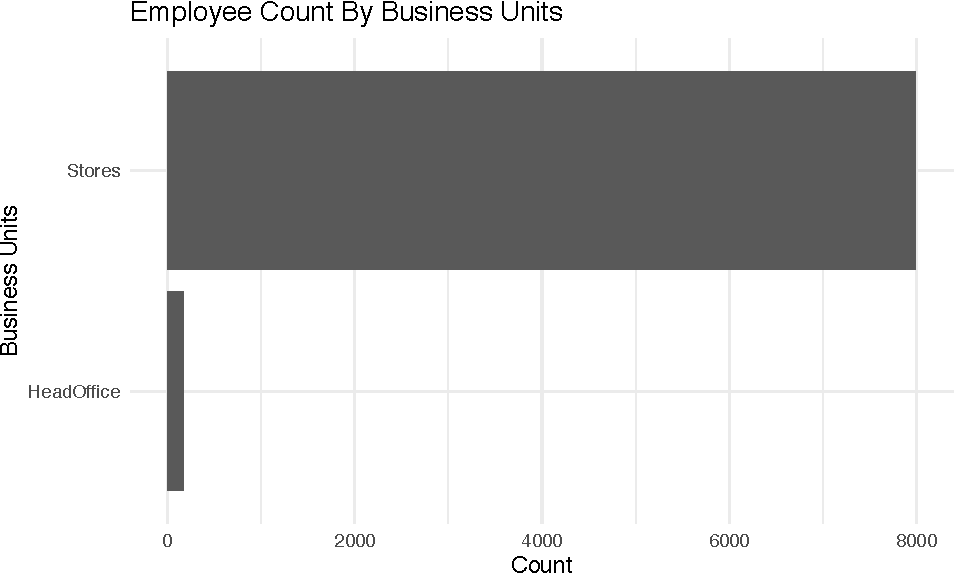
\includegraphics[width=\textwidth]{hendrikfeddersen_files/figure-latex/unnamed-chunk-7-1}

\begin{Shaded}
\begin{Highlighting}[]
\NormalTok{MFGEmployees }\OperatorTok\StringTok{ }
\StringTok{  }\KeywordTok{ggplot}\NormalTok{() }\OperatorTok{+}\StringTok{ }
\StringTok{  }\KeywordTok{aes}\NormalTok{(}\DataTypeTok{x=}\NormalTok{Gender) }\OperatorTok{+}\StringTok{ }
\StringTok{  }\KeywordTok{geom_bar}\NormalTok{() }\OperatorTok{+}
\StringTok{  }\KeywordTok{labs}\NormalTok{(}\DataTypeTok{x=}\StringTok{"Business Units"}\NormalTok{,}
       \DataTypeTok{y=}\StringTok{"Count"}\NormalTok{,}
       \DataTypeTok{title=}\StringTok{"Employee Count By Gender"}\NormalTok{) }\OperatorTok{+}
\StringTok{  }\KeywordTok{theme_minimal}\NormalTok{() }\OperatorTok{+}\StringTok{ }
\StringTok{  }\KeywordTok{coord_flip}\NormalTok{()}
\end{Highlighting}
\end{Shaded}

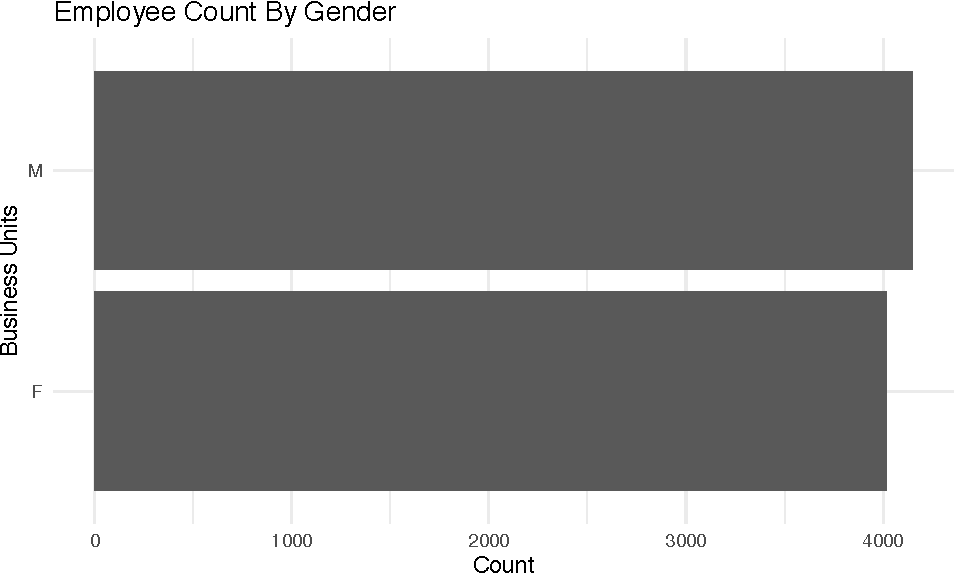
\includegraphics[width=\textwidth]{hendrikfeddersen_files/figure-latex/unnamed-chunk-7-2}

\begin{Shaded}
\begin{Highlighting}[]
\NormalTok{MFGEmployees }\OperatorTok\StringTok{ }
\StringTok{  }\KeywordTok{ggplot}\NormalTok{() }\OperatorTok{+}\StringTok{ }
\StringTok{  }\KeywordTok{aes}\NormalTok{(}\DataTypeTok{x=}\NormalTok{Division) }\OperatorTok{+}\StringTok{ }
\StringTok{  }\KeywordTok{geom_bar}\NormalTok{() }\OperatorTok{+}
\StringTok{  }\KeywordTok{labs}\NormalTok{(}\DataTypeTok{x=}\StringTok{"Division"}\NormalTok{,}
       \DataTypeTok{y=}\StringTok{"Count"}\NormalTok{,}
       \DataTypeTok{title=}\StringTok{"Employee Count By Division"}\NormalTok{) }\OperatorTok{+}
\StringTok{  }\KeywordTok{theme_minimal}\NormalTok{() }\OperatorTok{+}\StringTok{ }
\StringTok{  }\KeywordTok{coord_flip}\NormalTok{()}
\end{Highlighting}
\end{Shaded}

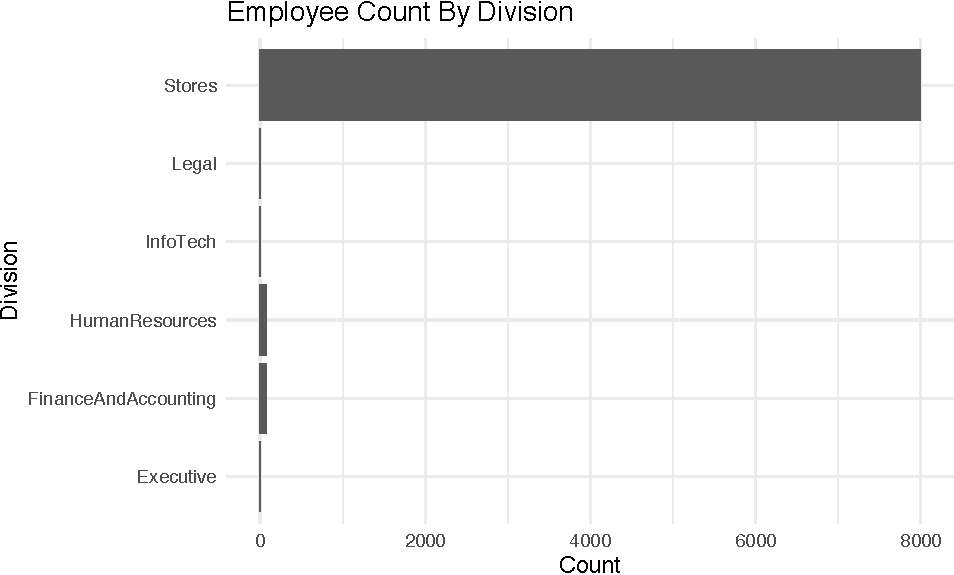
\includegraphics[width=\textwidth]{hendrikfeddersen_files/figure-latex/unnamed-chunk-7-3}

Let's ask some of our questions answered through this exploratory analysis.

\textbf{First of all, what is our absenteeism rate?}

\begin{Shaded}
\begin{Highlighting}[]
\NormalTok{MFGEmployees }\OperatorTok
\StringTok{  }\KeywordTok{summarise}\NormalTok{(}\DataTypeTok{median =} \KeywordTok{median}\NormalTok{(AbsenceRate), }\DataTypeTok{mean =} \KeywordTok{mean}\NormalTok{(AbsenceRate)) }\CommentTok{#Average absence rate and number of observations}
\end{Highlighting}
\end{Shaded}

\begin{verbatim}
## # A tibble: 1 x 2
##   median  mean
##    <dbl> <dbl>
## 1   2.69  2.91
\end{verbatim}

\begin{Shaded}
\begin{Highlighting}[]
\NormalTok{means <-}\StringTok{ }\KeywordTok{aggregate}\NormalTok{(AbsenceRate }\OperatorTok{~}\StringTok{ }\DecValTok{1}\NormalTok{, MFGEmployees, mean)}

\KeywordTok{ggplot}\NormalTok{() }\OperatorTok{+}\StringTok{ }
\StringTok{  }\KeywordTok{geom_boxplot}\NormalTok{(}\KeywordTok{aes}\NormalTok{(}\DataTypeTok{y =}\NormalTok{ AbsenceRate, }\DataTypeTok{x =}\DecValTok{1}\NormalTok{), }\DataTypeTok{data =}\NormalTok{ MFGEmployees) }\OperatorTok{+}
\StringTok{  }\KeywordTok{coord_flip}\NormalTok{() }\OperatorTok{+}
\StringTok{  }\KeywordTok{geom_text}\NormalTok{(}\DataTypeTok{data =} \KeywordTok{round}\NormalTok{(means, }\DataTypeTok{digits =} \DecValTok{3}\NormalTok{), }\KeywordTok{aes}\NormalTok{(}\DataTypeTok{y =}\NormalTok{ AbsenceRate, }\DataTypeTok{x =}\DecValTok{1}\NormalTok{, }\DataTypeTok{label =}\NormalTok{ AbsenceRate),  }\DataTypeTok{check_overlap=}\OtherTok{TRUE}\NormalTok{) }\OperatorTok{+}\StringTok{ }\CommentTok{#Add average absence rate as a text}
\StringTok{  }\KeywordTok{theme_minimal}\NormalTok{()}
\end{Highlighting}
\end{Shaded}

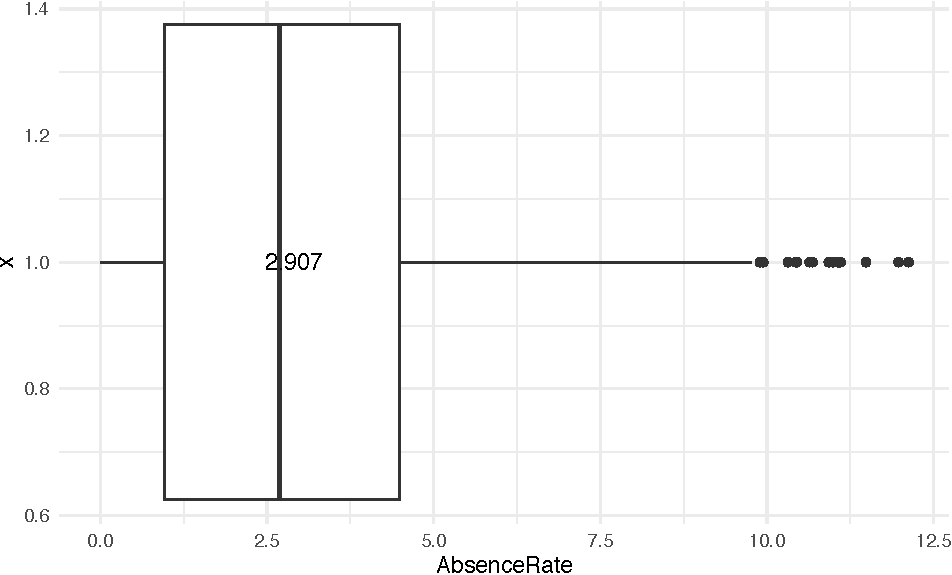
\includegraphics[width=\textwidth]{hendrikfeddersen_files/figure-latex/unnamed-chunk-8-1}
The average absence rate is `r scales::percent(mean(MFGEmployees\$AbsenceRate)'.

\textbf{Does anyone have excessive absenteeism?}

The boxplot shows the average (three digit number), the mean and standard deviation (through lines) of the data. Any observations beyond 3 standard deviations shows up as dots. So at least under that definition of outliers, some people show way more absenteeism than 99\% of employees.

\textbf{Does it vary across the organization?}

When you conduct a piece of quantitative research, you are inevitably attempting to answer a research question or hypothesis that you have set. One method of evaluating this research question is via a process called hypothesis testing, which is sometimes also referred to as significance testing.

In order to undertake hypothesis testing you need to express your research hypothesis as a null and alternative hypothesis. The null hypothesis and alternative hypothesis are statements regarding the differences or effects that occur in the population. You will use your sample to test which statement (i.e., the null hypothesis or alternative hypothesis) is most likely (although technically, you test the evidence against the null hypothesis). So, with respect to our example, the null and alternative hypothesis will reflect statements about absences among the organization.

In the following we will use ANOVA, as statistical test.

\begin{Shaded}
\begin{Highlighting}[]
\KeywordTok{ggplot}\NormalTok{() }\OperatorTok{+}\StringTok{ }
\StringTok{  }\KeywordTok{geom_boxplot}\NormalTok{(}\KeywordTok{aes}\NormalTok{(}\DataTypeTok{y =}\NormalTok{ AbsenceRate, }\DataTypeTok{x =}\NormalTok{ Gender), }\DataTypeTok{data =}\NormalTok{ MFGEmployees) }\OperatorTok{+}\StringTok{ }
\StringTok{  }\KeywordTok{coord_flip}\NormalTok{() }\OperatorTok{+}
\StringTok{  }\KeywordTok{theme_minimal}\NormalTok{()}
\end{Highlighting}
\end{Shaded}

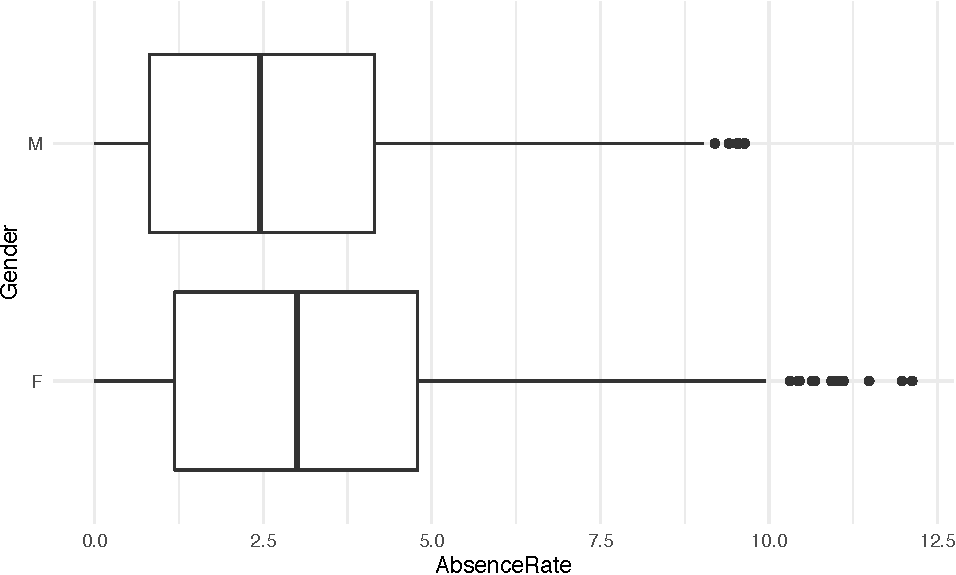
\includegraphics[width=\textwidth]{hendrikfeddersen_files/figure-latex/unnamed-chunk-9-1}

\begin{Shaded}
\begin{Highlighting}[]
\NormalTok{AnovaModel}\FloatTok{.1}\NormalTok{ <-}\StringTok{ }\KeywordTok{lm}\NormalTok{(AbsenceRate }\OperatorTok{~}\StringTok{ }\NormalTok{Gender, }\DataTypeTok{data=}\NormalTok{MFGEmployees) }\OperatorTok\StringTok{ }
\StringTok{  }\KeywordTok{Anova}\NormalTok{()}

\NormalTok{AnovaModel}\FloatTok{.1} 
\end{Highlighting}
\end{Shaded}

\begin{verbatim}
## Anova Table (Type II tests)
## 
## Response: AbsenceRate
##           Sum Sq   Df F value              Pr(>F)    
## Gender       496    1    97.8 <0.0000000000000002 ***
## Residuals  41379 8163                                
## ---
## Signif. codes:  0 '***' 0.001 '**' 0.01 '*' 0.05 '.' 0.1 ' ' 1
\end{verbatim}

\begin{Shaded}
\begin{Highlighting}[]
\CommentTok{#means}
\NormalTok{MFGEmployees }\OperatorTok\StringTok{ }\KeywordTok{group_by}\NormalTok{(Gender) }\OperatorTok\StringTok{ }\KeywordTok{summarise}\NormalTok{(}\DataTypeTok{avg=}\KeywordTok{mean}\NormalTok{(AbsenceRate))}
\end{Highlighting}
\end{Shaded}

\begin{verbatim}
## # A tibble: 2 x 2
##   Gender   avg
##   <chr>  <dbl>
## 1 F       3.16
## 2 M       2.66
\end{verbatim}

The output of the function is a classical ANOVA table with the following data:
Df = degree of freedom
Sum Sq = deviance (within groups, and residual)
Mean Sq = variance (within groups, and residual)
F value = the value of the Fisher statistic test, so computed (variance within groups) / (variance residual)
Pr(\textgreater{}F) = p-value

Please note that the value 2.2e-16 actually means 2.2 X 10 \^{} -16. It is just a way R prints numbers that are either too big or too small.

Since the p-Value is much less than 0.05, we reject the null hypothesis and accept the alternative hypothesis, i.e.~the absence levels among are significantly different among genders.

\begin{Shaded}
\begin{Highlighting}[]
\KeywordTok{ggplot}\NormalTok{() }\OperatorTok{+}\StringTok{ }
\StringTok{  }\KeywordTok{geom_boxplot}\NormalTok{(}\KeywordTok{aes}\NormalTok{(}\DataTypeTok{y =}\NormalTok{ AbsenceRate, }\DataTypeTok{x =}\NormalTok{ Division), }\DataTypeTok{data =}\NormalTok{ MFGEmployees) }\OperatorTok{+}\StringTok{ }
\StringTok{  }\KeywordTok{coord_flip}\NormalTok{() }\OperatorTok{+}
\StringTok{  }\KeywordTok{theme_minimal}\NormalTok{()}
\end{Highlighting}
\end{Shaded}

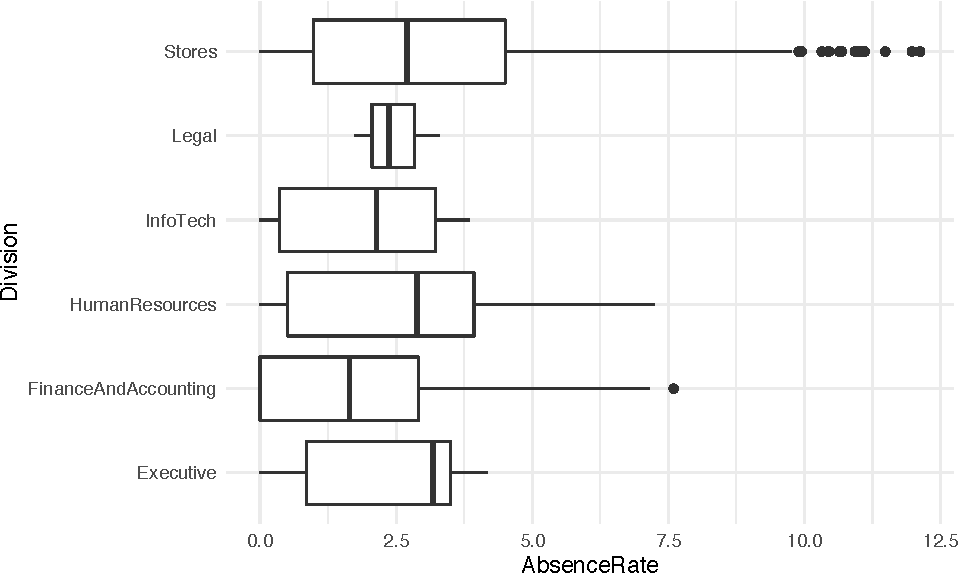
\includegraphics[width=\textwidth]{hendrikfeddersen_files/figure-latex/unnamed-chunk-10-1}

\begin{Shaded}
\begin{Highlighting}[]
\NormalTok{AnovaModel}\FloatTok{.2}\NormalTok{ <-}\StringTok{ }\KeywordTok{lm}\NormalTok{(AbsenceRate }\OperatorTok{~}\StringTok{ }\NormalTok{Division, }\DataTypeTok{data=}\NormalTok{MFGEmployees) }\OperatorTok\StringTok{ }
\StringTok{  }\KeywordTok{Anova}\NormalTok{()}

\NormalTok{AnovaModel}\FloatTok{.2}
\end{Highlighting}
\end{Shaded}

\begin{verbatim}
## Anova Table (Type II tests)
## 
## Response: AbsenceRate
##           Sum Sq   Df F value Pr(>F)   
## Division      91    5    3.56 0.0032 **
## Residuals  41783 8159                  
## ---
## Signif. codes:  0 '***' 0.001 '**' 0.01 '*' 0.05 '.' 0.1 ' ' 1
\end{verbatim}

\begin{Shaded}
\begin{Highlighting}[]
\CommentTok{# means}
\NormalTok{MFGEmployees }\OperatorTok\StringTok{ }\KeywordTok{group_by}\NormalTok{(Division) }\OperatorTok\StringTok{ }\KeywordTok{summarise}\NormalTok{(}\DataTypeTok{avg=}\KeywordTok{mean}\NormalTok{(AbsenceRate))}
\end{Highlighting}
\end{Shaded}

\begin{verbatim}
## # A tibble: 6 x 2
##   Division               avg
##   <chr>                <dbl>
## 1 Executive             2.32
## 2 FinanceAndAccounting  1.92
## 3 HumanResources        2.65
## 4 InfoTech              1.93
## 5 Legal                 2.47
## 6 Stores                2.92
\end{verbatim}

The absence levels among are significantly different among Division.

\begin{Shaded}
\begin{Highlighting}[]
\NormalTok{AnovaModel}\FloatTok{.3}\NormalTok{ <-}\StringTok{ }\KeywordTok{lm}\NormalTok{(AbsenceRate }\OperatorTok{~}\StringTok{ }\NormalTok{Division}\OperatorTok{*}\NormalTok{Gender, }\DataTypeTok{data=}\NormalTok{MFGEmployees) }\OperatorTok\StringTok{ }
\StringTok{  }\KeywordTok{Anova}\NormalTok{()}

\NormalTok{AnovaModel}\FloatTok{.3}
\end{Highlighting}
\end{Shaded}

\begin{verbatim}
## Anova Table (Type II tests)
## 
## Response: AbsenceRate
##                 Sum Sq   Df F value              Pr(>F)    
## Division            92    5    3.61              0.0029 ** 
## Gender             496    1   97.94 <0.0000000000000002 ***
## Division:Gender      5    5    0.18              0.9708    
## Residuals        41283 8153                                
## ---
## Signif. codes:  0 '***' 0.001 '**' 0.01 '*' 0.05 '.' 0.1 ' ' 1
\end{verbatim}

\begin{Shaded}
\begin{Highlighting}[]
\CommentTok{#means}
\NormalTok{MFGEmployees }\OperatorTok\StringTok{ }\KeywordTok{group_by}\NormalTok{(Division, Gender) }\OperatorTok\StringTok{ }\KeywordTok{summarise}\NormalTok{(}\DataTypeTok{avg=}\KeywordTok{mean}\NormalTok{(AbsenceRate))}
\end{Highlighting}
\end{Shaded}

\begin{verbatim}
## # A tibble: 12 x 3
## # Groups:   Division [6]
##    Division             Gender   avg
##    <chr>                <chr>  <dbl>
##  1 Executive            F       2.98
##  2 Executive            M       1.78
##  3 FinanceAndAccounting F       2.17
##  4 FinanceAndAccounting M       1.63
##  5 HumanResources       F       3.01
##  6 HumanResources       M       2.21
##  7 InfoTech             F       3.30
##  8 InfoTech             M       1.77
##  9 Legal                F       3.30
## 10 Legal                M       2.06
## 11 Stores               F       3.17
## 12 Stores               M       2.68
\end{verbatim}

If varies significantly by the interaction of gender and division.

These are just a handful of the categorical summaries we could do.

\textbf{Does AbsenceRate vary by length of service and age?}

Scatterplots and correlations help answer this.

\begin{Shaded}
\begin{Highlighting}[]
\CommentTok{# basic scatterplot}
\NormalTok{MFGEmployees }\OperatorTok
\KeywordTok{ggplot}\NormalTok{() }\OperatorTok{+}
\StringTok{  }\KeywordTok{aes}\NormalTok{(}\DataTypeTok{x=}\NormalTok{Age, }\DataTypeTok{y=}\NormalTok{AbsenceRate) }\OperatorTok{+}\StringTok{ }
\StringTok{  }\KeywordTok{geom_point}\NormalTok{(}\DataTypeTok{colour =} \StringTok{"blue"}\NormalTok{) }\OperatorTok{+}
\StringTok{  }\KeywordTok{theme_minimal}\NormalTok{()}
\end{Highlighting}
\end{Shaded}

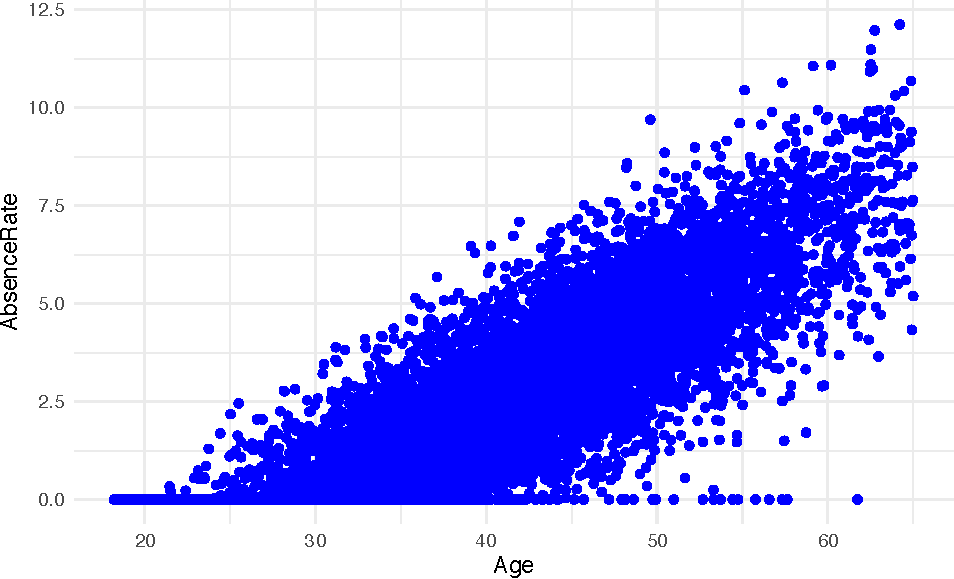
\includegraphics[width=\textwidth]{hendrikfeddersen_files/figure-latex/unnamed-chunk-12-1}

\begin{Shaded}
\begin{Highlighting}[]
\KeywordTok{cor}\NormalTok{(MFGEmployees}\OperatorTok{$}\NormalTok{Age, MFGEmployees}\OperatorTok{$}\NormalTok{AbsenceRate)}
\end{Highlighting}
\end{Shaded}

\begin{verbatim}
## [1] 0.825
\end{verbatim}

There is a strong correlation of Age and Absence Rate

\begin{Shaded}
\begin{Highlighting}[]
\NormalTok{MFGEmployees }\OperatorTok
\KeywordTok{ggplot}\NormalTok{() }\OperatorTok{+}
\StringTok{  }\KeywordTok{aes}\NormalTok{(}\DataTypeTok{x=}\NormalTok{LengthService, }\DataTypeTok{y=}\NormalTok{AbsenceRate) }\OperatorTok{+}\StringTok{ }
\StringTok{  }\KeywordTok{geom_point}\NormalTok{(}\DataTypeTok{colour =} \StringTok{"blue"}\NormalTok{) }\OperatorTok{+}
\StringTok{  }\KeywordTok{geom_smooth}\NormalTok{(}\DataTypeTok{method=}\StringTok{'lm'}\NormalTok{, }\DataTypeTok{se =} \OtherTok{FALSE}\NormalTok{, }\DataTypeTok{color=}\StringTok{'red'}\NormalTok{) }\OperatorTok{+}
\StringTok{  }\KeywordTok{theme_minimal}\NormalTok{()}
\end{Highlighting}
\end{Shaded}

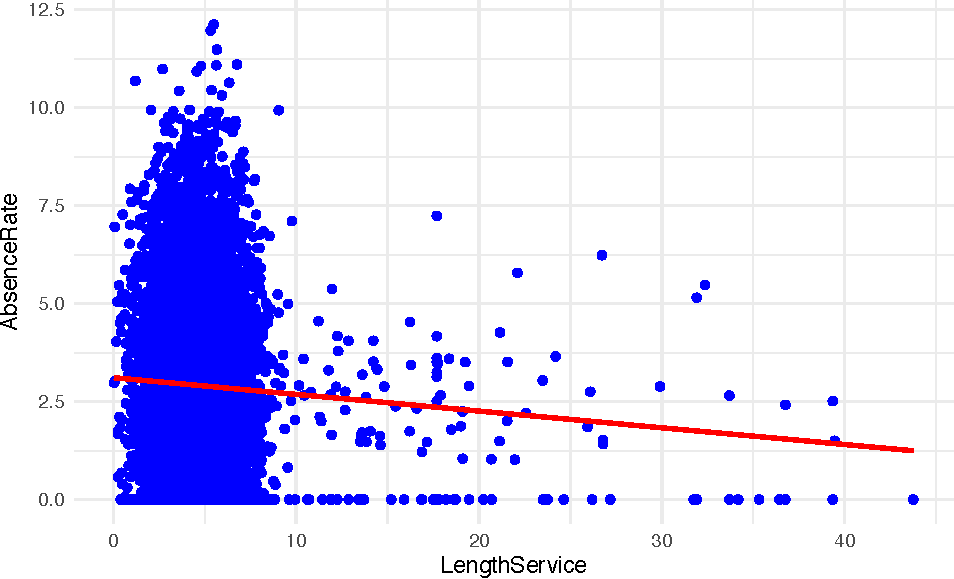
\includegraphics[width=\textwidth]{hendrikfeddersen_files/figure-latex/unnamed-chunk-13-1}

\begin{Shaded}
\begin{Highlighting}[]
\KeywordTok{cor}\NormalTok{(MFGEmployees}\OperatorTok{$}\NormalTok{LengthService, MFGEmployees}\OperatorTok{$}\NormalTok{AbsenceRate)}
\end{Highlighting}
\end{Shaded}

\begin{verbatim}
## [1] -0.0467
\end{verbatim}

There is not a strong correlation between length of service and Absence Rate.

\begin{Shaded}
\begin{Highlighting}[]
\NormalTok{MFGEmployees }\OperatorTok
\KeywordTok{ggplot}\NormalTok{() }\OperatorTok{+}
\StringTok{  }\KeywordTok{aes}\NormalTok{(}\DataTypeTok{x=}\NormalTok{Age, }\DataTypeTok{y=}\NormalTok{LengthService) }\OperatorTok{+}\StringTok{ }
\StringTok{  }\KeywordTok{geom_point}\NormalTok{(}\DataTypeTok{colour =} \StringTok{"blue"}\NormalTok{) }\OperatorTok{+}
\StringTok{  }\KeywordTok{geom_smooth}\NormalTok{(}\DataTypeTok{method=}\StringTok{'lm'}\NormalTok{, }\DataTypeTok{se =} \OtherTok{FALSE}\NormalTok{, }\DataTypeTok{color=}\StringTok{'red'}\NormalTok{) }\OperatorTok{+}
\StringTok{  }\KeywordTok{theme_minimal}\NormalTok{()}
\end{Highlighting}
\end{Shaded}

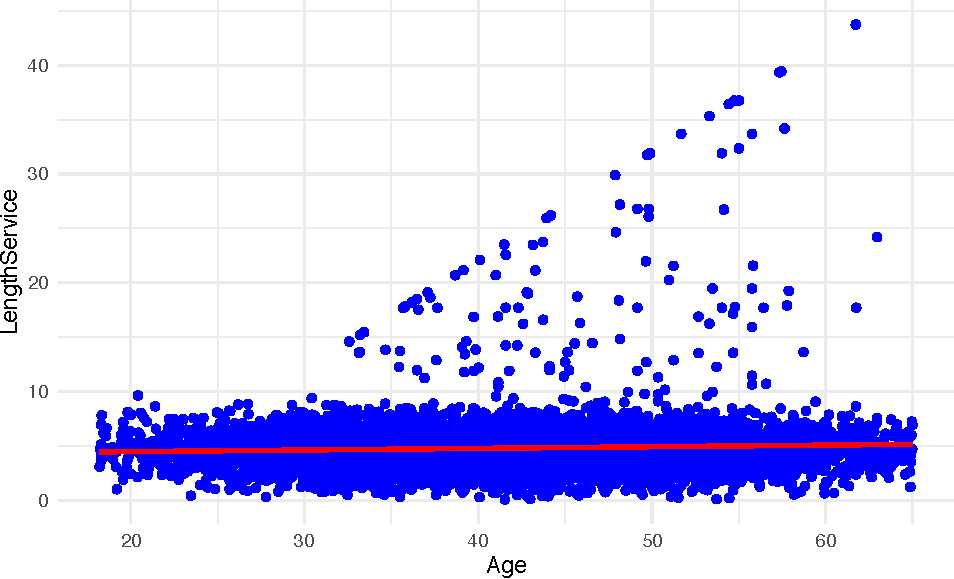
\includegraphics[width=\textwidth]{hendrikfeddersen_files/figure-latex/unnamed-chunk-14-1}

\begin{Shaded}
\begin{Highlighting}[]
\KeywordTok{cor}\NormalTok{(MFGEmployees}\OperatorTok{$}\NormalTok{Age, MFGEmployees}\OperatorTok{$}\NormalTok{LengthService)}
\end{Highlighting}
\end{Shaded}

\begin{verbatim}
## [1] 0.0562
\end{verbatim}

There is not much correlation between age and length of service either.

So far, we have done data exploration, now we are going to start building a model and starting to answer more difficult questions.

\#\#3. Build The model
One of the questions asked in the defining the goal step was `whether it was possible to \textbf{predict} absenteeism?'

Absence Rate is a numeric continuous value. In the `Building a model' step we have to chose which models/statistical algorithms to use. Prediction of a numerics continous values suggests a couple of models that could be brought to bear: Regression trees and linear regression. There are many more but for purposes of this article we will look at these.

\#\#\#3.1 Regression Trees
Regression Trees will allow for use of both categorical and numeric values as predictors. Let's choose the following data as potential predictors in this analysis:

\begin{itemize}
\tightlist
\item
  Gender
\item
  Department Name
\item
  Store Location
\item
  Division
\item
  Age
\item
  Length of Service
\item
  Business Unit
\end{itemize}

\textbf{Absence Rate} will be the the `target' or thing to be predicted.

\begin{Shaded}
\begin{Highlighting}[]
\NormalTok{MYinput <-}\StringTok{ }\KeywordTok{c}\NormalTok{(}\StringTok{"Gender"}\NormalTok{, }\StringTok{"DepartmentName"}\NormalTok{, }\StringTok{"StoreLocation"}\NormalTok{, }\StringTok{"Division"}\NormalTok{,}
             \StringTok{"Age"}\NormalTok{, }\StringTok{"LengthService"}\NormalTok{, }\StringTok{"BusinessUnit"}\NormalTok{)}
\NormalTok{MYtarget  <-}\StringTok{ "AbsenceRate"}

\KeywordTok{library}\NormalTok{(rpart, }\DataTypeTok{quietly=}\OtherTok{TRUE}\NormalTok{)}

\KeywordTok{set.seed}\NormalTok{(crv}\OperatorTok{$}\NormalTok{seed)}
\NormalTok{MYrpart <-}\StringTok{ }\KeywordTok{rpart}\NormalTok{(AbsenceRate }\OperatorTok{~}\StringTok{ }\NormalTok{.,}
                 \DataTypeTok{data=}\NormalTok{MFGEmployees[, }\KeywordTok{c}\NormalTok{(MYinput, MYtarget)],}
                 \DataTypeTok{method=}\StringTok{"anova"}\NormalTok{,}
                 \DataTypeTok{parms=}\KeywordTok{list}\NormalTok{(}\DataTypeTok{split=}\StringTok{"information"}\NormalTok{),}
                 \DataTypeTok{control=}\KeywordTok{rpart.control}\NormalTok{(}\DataTypeTok{minsplit=}\DecValTok{10}\NormalTok{,}
                                       \DataTypeTok{maxdepth=}\DecValTok{10}\NormalTok{,}
                                       \DataTypeTok{usesurrogate=}\DecValTok{0}\NormalTok{, }
                                       \DataTypeTok{maxsurrogate=}\DecValTok{0}\NormalTok{))}

\KeywordTok{fancyRpartPlot}\NormalTok{(MYrpart, }\DataTypeTok{main=}\StringTok{"Decision Tree MFGEmployees and AbsenceRate"}\NormalTok{)}
\end{Highlighting}
\end{Shaded}

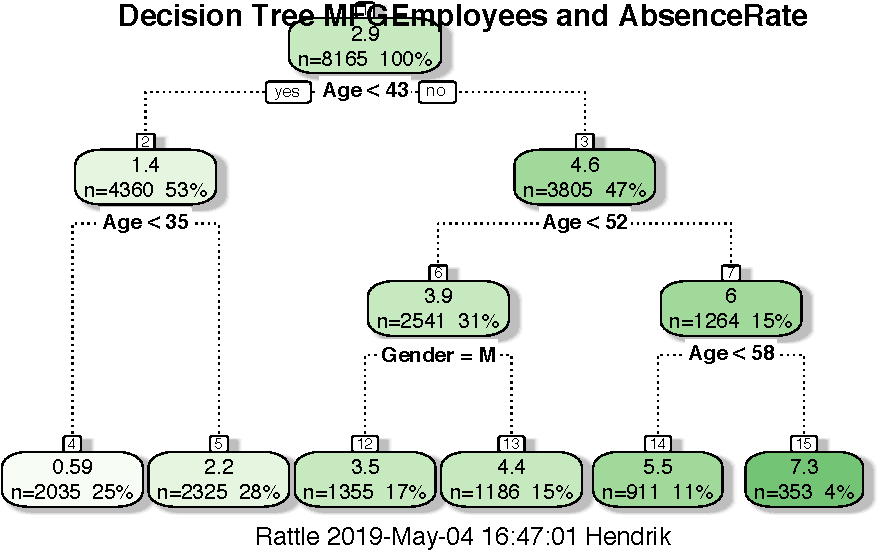
\includegraphics[width=\textwidth]{hendrikfeddersen_files/figure-latex/unnamed-chunk-15-1}

The regression decision tree shows that age is a big factor in determining absence rate with gender playing a small part in one of the age ranges: \textgreater{}43 and \textless{}52 with males having a lower absence rate in this group. Almost all categorical information other than gender doesn't look like to help in the prediction.

Now let's look at linear regression as another model. The restriction in linear regression is that it can only accept non-categorical variables. Categorical variables can sometimes be made numeric through transformation, but that is beyond the scope of this article.

\#\#\#3.2 Linear Regression

In linear regression, then, we will need to restrict it to numeric variables:

\begin{itemize}
\tightlist
\item
  Age
\item
  Length of Service
\end{itemize}

being used to predict absence rate.

\begin{Shaded}
\begin{Highlighting}[]
\CommentTok{#Linear Regression Model}
\NormalTok{RegressionCurrentData <-}\StringTok{ }\KeywordTok{lm}\NormalTok{(AbsenceRate}\OperatorTok{~}\NormalTok{Age}\OperatorTok{+}\NormalTok{LengthService, }\DataTypeTok{data=}\NormalTok{MFGEmployees)}

\KeywordTok{summary}\NormalTok{(RegressionCurrentData)}
\end{Highlighting}
\end{Shaded}

\begin{verbatim}
## 
## Call:
## lm(formula = AbsenceRate ~ Age + LengthService, data = MFGEmployees)
## 
## Residuals:
##    Min     1Q Median     3Q    Max 
## -5.358 -0.847 -0.023  0.852  5.103 
## 
## Coefficients:
##               Estimate Std. Error t value            Pr(>|t|)    
## (Intercept)   -5.19021    0.06896   -75.3 <0.0000000000000002 ***
## Age            0.20259    0.00151   134.2 <0.0000000000000002 ***
## LengthService -0.08531    0.00565   -15.1 <0.0000000000000002 ***
## ---
## Signif. codes:  0 '***' 0.001 '**' 0.01 '*' 0.05 '.' 0.1 ' ' 1
## 
## Residual standard error: 1.26 on 8162 degrees of freedom
## Multiple R-squared:  0.689,  Adjusted R-squared:  0.689 
## F-statistic: 9.03e+03 on 2 and 8162 DF,  p-value: <0.0000000000000002
\end{verbatim}

The summary shows an adjusted R-squared of 0.689 which means approximately 68.9\% of the variance is accounted by age and length of service.
The variables are both significant at Pr(\textgreater{}\textbar{}t\textbar{}) of 'r summary(RegressionCurrentData)\$coefficients{[}3,4{]}`. These results are using the entirety of the existing data to predict itself.

Graphically it look like this:

\begin{Shaded}
\begin{Highlighting}[]
\CommentTok{#2D plot of Age and AbsenceRate}

\KeywordTok{ggplot}\NormalTok{() }\OperatorTok{+}\StringTok{ }
\StringTok{  }\KeywordTok{geom_point}\NormalTok{(}\KeywordTok{aes}\NormalTok{(}\DataTypeTok{x =}\NormalTok{ Age,}\DataTypeTok{y =}\NormalTok{ AbsenceRate),}\DataTypeTok{data=}\NormalTok{MFGEmployees) }\OperatorTok{+}
\StringTok{  }\KeywordTok{geom_smooth}\NormalTok{(}\KeywordTok{aes}\NormalTok{(}\DataTypeTok{x =}\NormalTok{ Age,}\DataTypeTok{y =}\NormalTok{ AbsenceRate),}\DataTypeTok{data=}\NormalTok{MFGEmployees,}\DataTypeTok{method =} \StringTok{'lm'}\NormalTok{) }\OperatorTok{+}
\StringTok{  }\KeywordTok{theme_minimal}\NormalTok{()}
\end{Highlighting}
\end{Shaded}

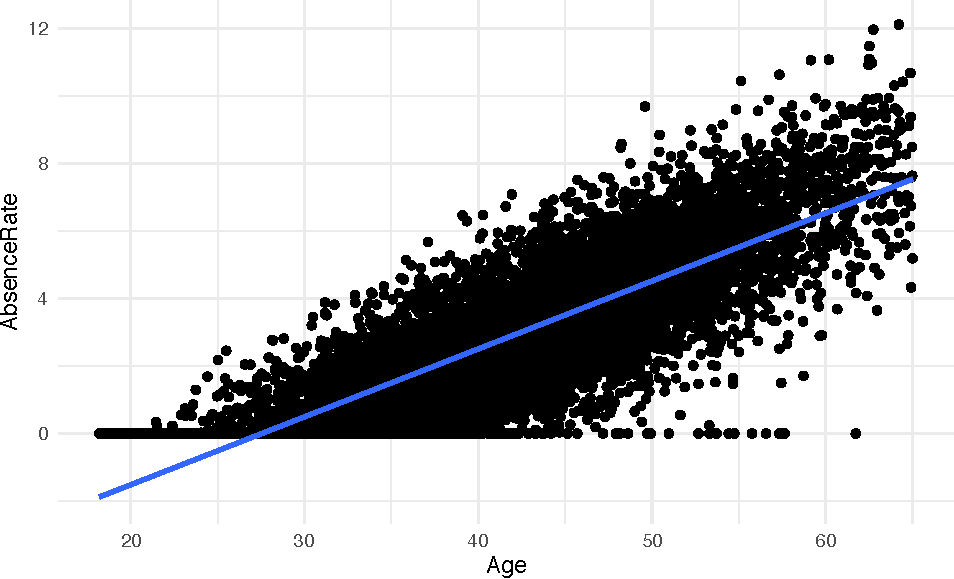
\includegraphics[width=\textwidth]{hendrikfeddersen_files/figure-latex/unnamed-chunk-17-1}

\begin{Shaded}
\begin{Highlighting}[]
\CommentTok{#3D Scatterplot  of Age and Length of Service with Absence Rate - with Coloring and Vertical Lines}
\CommentTok{# and Regression Plane }
\KeywordTok{library}\NormalTok{(scatterplot3d) }

\NormalTok{s3d <-}\KeywordTok{scatterplot3d}\NormalTok{(MFGEmployees}\OperatorTok{$}\NormalTok{Age,MFGEmployees}\OperatorTok{$}\NormalTok{LengthService,MFGEmployees}\OperatorTok{$}\NormalTok{AbsenceRate, }\DataTypeTok{pch=}\DecValTok{16}\NormalTok{, }\DataTypeTok{highlight.3d=}\OtherTok{TRUE}\NormalTok{,}
                    \DataTypeTok{type=}\StringTok{"h"}\NormalTok{, }\DataTypeTok{main=}\StringTok{"Absence Rate By Age And Length of Service"}\NormalTok{)}
\NormalTok{fit <-}\StringTok{ }\KeywordTok{lm}\NormalTok{(MFGEmployees}\OperatorTok{$}\NormalTok{AbsenceRate }\OperatorTok{~}\StringTok{ }\NormalTok{MFGEmployees}\OperatorTok{$}\NormalTok{Age}\OperatorTok{+}\NormalTok{MFGEmployees}\OperatorTok{$}\NormalTok{LengthService) }

\NormalTok{s3d}\OperatorTok{$}\KeywordTok{plane3d}\NormalTok{(fit)}
\end{Highlighting}
\end{Shaded}

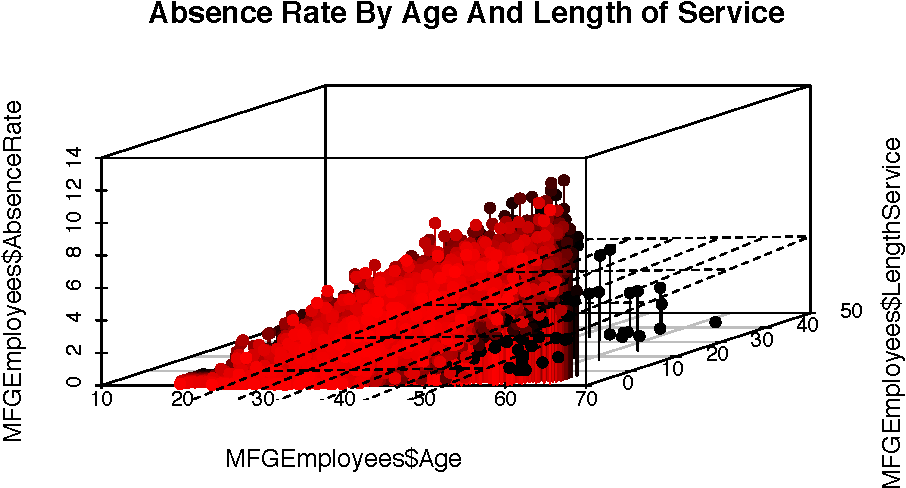
\includegraphics[width=\textwidth]{hendrikfeddersen_files/figure-latex/unnamed-chunk-17-2}

\#\#4.Evaluate and evaluate the model

Up till now we have concentrated on producing a couple of models. The effort so far has had one weakness. \textbf{We have used all of our data for 2015 to generate the models.} They can both predict, but the prediction are based on existing data - that are already known. We don't know how well it will predict on data it hasn't seen yet.

To evaluate and critique the models, we need to train the model using part of the data and hold out a portion to test on. We will divide the data into 10 parts- using 9 parts as training data and 1 part as testing data, and alternate which are the 9 and the 1, so that each of the 10 parts gets to be training data 9 times and testing data once.

The R ``caret'' library helps us do that. We will run both a regression tree and linear regression and compare how they do against each other.

First the Linear Regression

\begin{Shaded}
\begin{Highlighting}[]
\KeywordTok{library}\NormalTok{(caret)}

\KeywordTok{set.seed}\NormalTok{(}\DecValTok{998}\NormalTok{)}

\NormalTok{inTraining <-}\StringTok{ }\KeywordTok{createDataPartition}\NormalTok{(MFGEmployees}\OperatorTok{$}\NormalTok{BusinessUnit, }\DataTypeTok{p =} \FloatTok{.75}\NormalTok{, }\DataTypeTok{list =} \OtherTok{FALSE}\NormalTok{)}

\NormalTok{training <-}\StringTok{ }\NormalTok{MFGEmployees[inTraining,]}
\NormalTok{testing <-}\StringTok{ }\NormalTok{MFGEmployees[ }\OperatorTok{-}\StringTok{ }\NormalTok{inTraining,]}

\NormalTok{fitControl <-}\StringTok{ }\KeywordTok{trainControl}\NormalTok{(}\CommentTok{## 10-fold CV}
\DataTypeTok{method =} \StringTok{"repeatedcv"}\NormalTok{, }\DataTypeTok{number =} \DecValTok{10}\NormalTok{, }
\DataTypeTok{repeats =} \DecValTok{10} \CommentTok{## repeated ten times}
\NormalTok{)}

\KeywordTok{set.seed}\NormalTok{(}\DecValTok{825}\NormalTok{)}

\NormalTok{lmFit1 <-}\StringTok{ }\KeywordTok{train}\NormalTok{(AbsenceRate }\OperatorTok{~}\StringTok{ }\NormalTok{Age }\OperatorTok{+}\StringTok{ }\NormalTok{LengthService, }\DataTypeTok{data =}\NormalTok{ training,}
                 \DataTypeTok{method =} \StringTok{"lm"}\NormalTok{,}
                 \DataTypeTok{trControl =}\NormalTok{ fitControl)}
\NormalTok{lmFit1}
\end{Highlighting}
\end{Shaded}

\begin{verbatim}
## Linear Regression 
## 
## 6124 samples
##    2 predictor
## 
## No pre-processing
## Resampling: Cross-Validated (10 fold, repeated 10 times) 
## Summary of sample sizes: 5512, 5512, 5511, 5512, 5512, 5511, ... 
## Resampling results:
## 
##   RMSE  Rsquared  MAE 
##   1.27  0.688     1.01
## 
## Tuning parameter 'intercept' was held constant at a value of TRUE
\end{verbatim}

\begin{Shaded}
\begin{Highlighting}[]
\NormalTok{Testingdatasetandpredictions <-}\StringTok{ }\NormalTok{testing }\OperatorTok\StringTok{ }\KeywordTok{add_predictions}\NormalTok{(lmFit1, }\DataTypeTok{type =} \StringTok{"raw"}\NormalTok{)}

\NormalTok{Testingdatasetandpredictions}\OperatorTok{$}\NormalTok{pred[Testingdatasetandpredictions}\OperatorTok{$}\NormalTok{pred}\OperatorTok{<}\DecValTok{0}\NormalTok{] <-}\StringTok{ }\DecValTok{0} \CommentTok{#Put a zero to all negative predictions}
\end{Highlighting}
\end{Shaded}

The Rsquared shows a value of 0.688 which means even with sampling different parts of the data on 10 fold cross validation the use of age and length of service seems to be pretty robust so far.

Next the decision tree. The first time with just the numeric variables.

\begin{Shaded}
\begin{Highlighting}[]
\KeywordTok{set.seed}\NormalTok{(}\DecValTok{825}\NormalTok{)}

\NormalTok{rpartFit1 <-}\StringTok{ }\KeywordTok{train}\NormalTok{(AbsenceRate }\OperatorTok{~}\StringTok{ }\NormalTok{Age }\OperatorTok{+}\StringTok{ }\NormalTok{LengthService, }\DataTypeTok{data =}\NormalTok{ training,}
                 \DataTypeTok{method =} \StringTok{"rpart"}\NormalTok{,}
                 \DataTypeTok{trControl =}\NormalTok{ fitControl,}
                 \DataTypeTok{maxdepth =} \DecValTok{5}\NormalTok{)}
\NormalTok{rpartFit1}
\end{Highlighting}
\end{Shaded}

\begin{verbatim}
## CART 
## 
## 6124 samples
##    2 predictor
## 
## No pre-processing
## Resampling: Cross-Validated (10 fold, repeated 10 times) 
## Summary of sample sizes: 5512, 5512, 5511, 5512, 5512, 5511, ... 
## Resampling results across tuning parameters:
## 
##   cp      RMSE  Rsquared  MAE 
##   0.0597  1.43  0.605     1.13
##   0.0884  1.55  0.531     1.26
##   0.4945  1.98  0.475     1.63
## 
## RMSE was used to select the optimal model using the smallest value.
## The final value used for the model was cp = 0.0597.
\end{verbatim}

You will notice that the decision tree with 10 fold cross validation didn't perform as well with an RSquared of approximately 0.60

The second time with the original categorical and numeric varibles used.

\begin{Shaded}
\begin{Highlighting}[]
\KeywordTok{set.seed}\NormalTok{(}\DecValTok{825}\NormalTok{)}

\NormalTok{rpartFit2 <-}\StringTok{ }\KeywordTok{train}\NormalTok{(AbsenceRate }\OperatorTok{~}\StringTok{ }\NormalTok{Gender }\OperatorTok{+}\StringTok{ }\NormalTok{DepartmentName }\OperatorTok{+}\StringTok{ }\NormalTok{StoreLocation }\OperatorTok{+}\StringTok{ }\NormalTok{Division }\OperatorTok{+}\StringTok{ }\NormalTok{Age }\OperatorTok{+}\StringTok{ }\NormalTok{LengthService }\OperatorTok{+}\StringTok{ }\NormalTok{BusinessUnit, }\DataTypeTok{data =}\NormalTok{ training,}
                 \DataTypeTok{method =} \StringTok{"rpart"}\NormalTok{,}
                 \DataTypeTok{trControl =}\NormalTok{ fitControl,}
                 \DataTypeTok{maxdepth =} \DecValTok{5}\NormalTok{)}

\NormalTok{rpartFit2}
\end{Highlighting}
\end{Shaded}

\begin{verbatim}
## CART 
## 
## 6124 samples
##    7 predictor
## 
## No pre-processing
## Resampling: Cross-Validated (10 fold, repeated 10 times) 
## Summary of sample sizes: 5512, 5512, 5511, 5512, 5512, 5511, ... 
## Resampling results across tuning parameters:
## 
##   cp      RMSE  Rsquared  MAE 
##   0.0597  1.43  0.605     1.13
##   0.0884  1.55  0.531     1.26
##   0.4945  1.98  0.475     1.63
## 
## RMSE was used to select the optimal model using the smallest value.
## The final value used for the model was cp = 0.0597.
\end{verbatim}

Here when you include all originally used vaiables in 10 fold cross validation, the Rsquared changed little and is still around 0.60.

So far, the linear regression is performing better.

\#\#5.Present Results and Document

The presenting of results and documenting is something that R helps in. You may not have realized it, but the R Markdown language has been used to create the full layout of these two blog articles. HTML,PDF and Word formats can be produced.

R Markdown allows the reader to see exactly what you having been doing, so that an independent person can replicate your results, to confirm what you have done. It shows the R code/commands, the statistical results and graphics, all is included in the Absenteeism-Part.Rmd file.

\#\#6.Deploy Model

Once you have evaluated your model(s) and chosen to use them, they need to be deployed so that they can be used. At the simplest level, `deploy' can mean using the `predict' function in R (where applicable) in conjunction with your model.

\textbf{Can it predict next year absenteeism?}

Let's predict the 2016 Absenteeism from the 2015 model.

If we make the simplifying assumption that nobody quits and nobody new comes in, we can take the 2015 data and add 1 to age and 1 to years of service for an approximation of new 2016 data before we get to 2016.

\begin{Shaded}
\begin{Highlighting}[]
\CommentTok{#Apply model}
\CommentTok{#Generate 2016 data}
\NormalTok{Absence2016Data<-MFGEmployees}
\NormalTok{Absence2016Data}\OperatorTok{$}\NormalTok{Age<-Absence2016Data}\OperatorTok{$}\NormalTok{Age}\OperatorTok{+}\DecValTok{1}
\NormalTok{Absence2016Data}\OperatorTok{$}\NormalTok{LengthService<-Absence2016Data}\OperatorTok{$}\NormalTok{LengthService}\OperatorTok{+}\DecValTok{1}

\NormalTok{Absence2016Data <-}\StringTok{ }\NormalTok{Absence2016Data }\OperatorTok\StringTok{ }\KeywordTok{add_predictions}\NormalTok{(lmFit1, }\DataTypeTok{type =} \StringTok{"raw"}\NormalTok{)}
\NormalTok{Absence2016Data}\OperatorTok{$}\NormalTok{pred[Absence2016Data}\OperatorTok{$}\NormalTok{pred}\OperatorTok{<}\DecValTok{0}\NormalTok{] <-}\StringTok{ }\DecValTok{0} \CommentTok{#Put a zero to all negative predictions}
\end{Highlighting}
\end{Shaded}

To get single estimate for 2016 we ask for mean of absence rate.

\begin{Shaded}
\begin{Highlighting}[]
\KeywordTok{mean}\NormalTok{(Absence2016Data}\OperatorTok{$}\NormalTok{pred)}
\end{Highlighting}
\end{Shaded}

\begin{verbatim}
## [1] 3.05
\end{verbatim}

\begin{Shaded}
\begin{Highlighting}[]
\KeywordTok{mean}\NormalTok{(MFGEmployees}\OperatorTok{$}\NormalTok{AbsenceRate)}
\end{Highlighting}
\end{Shaded}

\begin{verbatim}
## [1] 2.91
\end{verbatim}

The first figure above is the 2016 prediction, the second is the 2015 actual for comparison.

\textbf{If so, how well can it predict?}

As mentioned previously, about `r scales::percent(mean(MFGEmployees\$AbsenceRate)'. of the variation is accounted for in a linear regression model using age and length of service.

\textbf{Can we reduce our absenteeism?}

On the surface, only getting the age reduced and length of service increased will reduce absensteeism with this model.

Obviously, absenteeism is much more complex that just the rudimentary data we have collected. A serious look at this metric and problem would require more and different kinds of data. As mentioned before, the raw data used in this article and analysis is totally contrived to illustrate an example.

\hypertarget{absenteeism-data-absenteeism_datawork}{%
\chapter{\texorpdfstring{Absenteeism data \{\#\href{mailto:absenteeism_data@work}{\nolinkurl{absenteeism\_data@work}}\}}{Absenteeism data \{\#absenteeism\_data@work\}}}\label{absenteeism-data-absenteeism_datawork}}

Placeholder

\hypertarget{data-reading}{%
\section{Data reading}\label{data-reading}}

\hypertarget{accidents_at_work}{%
\chapter{Accidents at work}\label{accidents_at_work}}

Placeholder

\hypertarget{attrition}{%
\chapter{Attrition}\label{attrition}}

Here we introduce attrition.

\hypertarget{interview-attendance}{%
\chapter{Interview attendance problem}\label{interview-attendance}}

Placeholder

\hypertarget{data-reading-1}{%
\section{Data reading}\label{data-reading-1}}

\hypertarget{choosing-a-model}{%
\section{Choosing a model}\label{choosing-a-model}}

\hypertarget{ranking-medical_school}{%
\chapter{Ranking Medical Schools}\label{ranking-medical_school}}

Placeholder

\hypertarget{webscraping-linkedin}{%
\chapter{Webscraping LinkedIn}\label{webscraping-linkedin}}

Placeholder

\hypertarget{flexdashboards}{%
\chapter{HR dashboards}\label{flexdashboards}}

Here we introduce flexdashboards

\hypertarget{shiny}{%
\chapter{HR Analytics product with Shiny}\label{shiny}}

Shiny is a very powerful framework for building web applications based on R. It is out of the scope of this book to make a comprehensive introduction to Shiny (which is too big a topic). We recommend that readers who are not familiar with Shiny learn more about it from the website \url{https://shiny.rstudio.com} before reading this chapter.

Unlike the more traditional workflow of creating static reports, you can create documents that allow your readers to change the parameters underlying your analysis and see the results immediately in Shiny R Markdown documents. In the example shown in Figure \citet{ref}(fig:shiny), the histogram will be automatically updated to reflect the number of bins selected by the reader.

A picture is worth a thousand words, and a Shiny document can potentially show you a thousand pictures as you interact with it. The readers are no longer tied to the fixed analysis and conclusions in the report. They may explore other possibilities by themselves, and possibly make new discoveries or draw different conclusions.

\hypertarget{appendix-appendix}{%
\appendix \addcontentsline{toc}{chapter}{\appendixname}}


\hypertarget{appendixA}{%
\chapter{Statistical Background}\label{appendixA}}

Placeholder

\hypertarget{basic-statistical-terms}{%
\section{Basic statistical terms}\label{basic-statistical-terms}}

\hypertarget{mean}{%
\subsection{Mean}\label{mean}}

\hypertarget{median}{%
\subsection{Median}\label{median}}

\hypertarget{standard-deviation}{%
\subsection{Standard deviation}\label{standard-deviation}}

\hypertarget{five-number-summary}{%
\subsection{Five-number summary}\label{five-number-summary}}

\hypertarget{distribution}{%
\subsection{Distribution}\label{distribution}}

\hypertarget{outliers}{%
\subsection{Outliers}\label{outliers}}

\hypertarget{normal-curve}{%
\section{Normal distribution}\label{normal-curve}}

\hypertarget{appendixB}{%
\chapter{Inference Examples}\label{appendixB}}

Placeholder

\hypertarget{needed-packages-10}{%
\section*{Needed packages}\label{needed-packages-10}}


\hypertarget{inference-mind-map}{%
\section{Inference mind map}\label{inference-mind-map}}

\hypertarget{one-mean}{%
\section{One mean}\label{one-mean}}

\hypertarget{problem-statement}{%
\subsection{Problem statement}\label{problem-statement}}

\hypertarget{competing-hypotheses}{%
\subsection{Competing hypotheses}\label{competing-hypotheses}}

\hypertarget{in-words}{%
\subsubsection*{In words}\label{in-words}}


\hypertarget{in-symbols-with-annotations}{%
\subsubsection*{In symbols (with annotations)}\label{in-symbols-with-annotations}}


\hypertarget{set-alpha}{%
\subsubsection*{\texorpdfstring{Set \(\alpha\)}{Set \textbackslash{}alpha}}\label{set-alpha}}


\hypertarget{exploring-the-sample-data}{%
\subsection{Exploring the sample data}\label{exploring-the-sample-data}}

\hypertarget{guess-about-statistical-significance}{%
\subsubsection*{Guess about statistical significance}\label{guess-about-statistical-significance}}


\hypertarget{non-traditional-methods}{%
\subsection{Non-traditional methods}\label{non-traditional-methods}}

\hypertarget{bootstrapping-for-hypothesis-test}{%
\subsubsection*{Bootstrapping for hypothesis test}\label{bootstrapping-for-hypothesis-test}}


\hypertarget{calculate-p-value}{%
\paragraph{\texorpdfstring{Calculate \(p\)-value}{Calculate p-value}}\label{calculate-p-value}}
\addcontentsline{toc}{paragraph}{Calculate \(p\)-value}

\hypertarget{bootstrapping-for-confidence-interval}{%
\subsubsection*{Bootstrapping for confidence interval}\label{bootstrapping-for-confidence-interval}}


\hypertarget{traditional-methods}{%
\subsection{Traditional methods}\label{traditional-methods}}

\hypertarget{check-conditions}{%
\subsubsection*{Check conditions}\label{check-conditions}}


\hypertarget{test-statistic}{%
\subsubsection*{Test statistic}\label{test-statistic}}


\hypertarget{observed-test-statistic}{%
\paragraph{Observed test statistic}\label{observed-test-statistic}}
\addcontentsline{toc}{paragraph}{Observed test statistic}

\hypertarget{compute-p-value}{%
\subsubsection*{\texorpdfstring{Compute \(p\)-value}{Compute p-value}}\label{compute-p-value}}


\hypertarget{state-conclusion}{%
\subsubsection*{State conclusion}\label{state-conclusion}}


\hypertarget{confidence-interval}{%
\subsubsection*{Confidence interval}\label{confidence-interval}}


\hypertarget{comparing-results}{%
\subsection{Comparing results}\label{comparing-results}}

\hypertarget{one-proportion}{%
\section{One proportion}\label{one-proportion}}

\hypertarget{problem-statement-1}{%
\subsection{Problem statement}\label{problem-statement-1}}

\hypertarget{competing-hypotheses-1}{%
\subsection{Competing hypotheses}\label{competing-hypotheses-1}}

\hypertarget{in-words-1}{%
\subsubsection*{In words}\label{in-words-1}}


\hypertarget{in-symbols-with-annotations-1}{%
\subsubsection*{In symbols (with annotations)}\label{in-symbols-with-annotations-1}}


\hypertarget{set-alpha-1}{%
\subsubsection*{\texorpdfstring{Set \(\alpha\)}{Set \textbackslash{}alpha}}\label{set-alpha-1}}


\hypertarget{exploring-the-sample-data-1}{%
\subsection{Exploring the sample data}\label{exploring-the-sample-data-1}}

\hypertarget{guess-about-statistical-significance-1}{%
\subsubsection*{Guess about statistical significance}\label{guess-about-statistical-significance-1}}


\hypertarget{non-traditional-methods-1}{%
\subsection{Non-traditional methods}\label{non-traditional-methods-1}}

\hypertarget{simulation-for-hypothesis-test}{%
\subsubsection*{Simulation for hypothesis test}\label{simulation-for-hypothesis-test}}


\hypertarget{calculate-p-value-1}{%
\paragraph{\texorpdfstring{Calculate \(p\)-value}{Calculate p-value}}\label{calculate-p-value-1}}
\addcontentsline{toc}{paragraph}{Calculate \(p\)-value}

\hypertarget{bootstrapping-for-confidence-interval-1}{%
\subsubsection*{Bootstrapping for confidence interval}\label{bootstrapping-for-confidence-interval-1}}


\hypertarget{traditional-methods-1}{%
\subsection{Traditional methods}\label{traditional-methods-1}}

\hypertarget{check-conditions-1}{%
\subsubsection*{Check conditions}\label{check-conditions-1}}


\hypertarget{test-statistic-1}{%
\subsubsection*{Test statistic}\label{test-statistic-1}}


\hypertarget{observed-test-statistic-1}{%
\paragraph{Observed test statistic}\label{observed-test-statistic-1}}
\addcontentsline{toc}{paragraph}{Observed test statistic}

\hypertarget{visualize-and-compute-p-value}{%
\subsubsection*{\texorpdfstring{Visualize and compute \(p\)-value}{Visualize and compute p-value}}\label{visualize-and-compute-p-value}}


\hypertarget{state-conclusion-1}{%
\subsubsection*{State conclusion}\label{state-conclusion-1}}


\hypertarget{comparing-results-1}{%
\subsection{Comparing results}\label{comparing-results-1}}

\hypertarget{two-proportions}{%
\section{Two proportions}\label{two-proportions}}

\hypertarget{problem-statement-2}{%
\subsection{Problem statement}\label{problem-statement-2}}

\hypertarget{competing-hypotheses-2}{%
\subsection{Competing hypotheses}\label{competing-hypotheses-2}}

\hypertarget{in-words-2}{%
\subsubsection*{In words}\label{in-words-2}}


\hypertarget{another-way-in-words}{%
\subsubsection*{Another way in words}\label{another-way-in-words}}


\hypertarget{in-symbols-with-annotations-2}{%
\subsubsection*{In symbols (with annotations)}\label{in-symbols-with-annotations-2}}


\hypertarget{set-alpha-2}{%
\subsubsection*{\texorpdfstring{Set \(\alpha\)}{Set \textbackslash{}alpha}}\label{set-alpha-2}}


\hypertarget{exploring-the-sample-data-2}{%
\subsection{Exploring the sample data}\label{exploring-the-sample-data-2}}

\hypertarget{guess-about-statistical-significance-2}{%
\subsubsection*{Guess about statistical significance}\label{guess-about-statistical-significance-2}}


\hypertarget{non-traditional-methods-2}{%
\subsection{Non-traditional methods}\label{non-traditional-methods-2}}

\hypertarget{collecting-summary-info}{%
\subsubsection*{Collecting summary info}\label{collecting-summary-info}}


\hypertarget{randomization-for-hypothesis-test}{%
\subsubsection*{Randomization for hypothesis test}\label{randomization-for-hypothesis-test}}


\hypertarget{calculate-p-value-2}{%
\paragraph{\texorpdfstring{Calculate \(p\)-value}{Calculate p-value}}\label{calculate-p-value-2}}
\addcontentsline{toc}{paragraph}{Calculate \(p\)-value}

\hypertarget{bootstrapping-for-confidence-interval-2}{%
\subsubsection*{Bootstrapping for confidence interval}\label{bootstrapping-for-confidence-interval-2}}


\hypertarget{traditional-methods-2}{%
\subsection{Traditional methods}\label{traditional-methods-2}}

\hypertarget{check-conditions-2}{%
\subsection{Check conditions}\label{check-conditions-2}}

\hypertarget{test-statistic-2}{%
\subsection{Test statistic}\label{test-statistic-2}}

\hypertarget{observed-test-statistic-2}{%
\subsubsection*{Observed test statistic}\label{observed-test-statistic-2}}


\hypertarget{state-conclusion-2}{%
\subsection{State conclusion}\label{state-conclusion-2}}

\hypertarget{comparing-results-2}{%
\subsection{Comparing results}\label{comparing-results-2}}

\hypertarget{two-means-independent-samples}{%
\section{Two means (independent samples)}\label{two-means-independent-samples}}

\hypertarget{problem-statement-3}{%
\subsection{Problem statement}\label{problem-statement-3}}

\hypertarget{competing-hypotheses-3}{%
\subsection{Competing hypotheses}\label{competing-hypotheses-3}}

\hypertarget{in-words-3}{%
\subsubsection*{In words}\label{in-words-3}}


\hypertarget{another-way-in-words-1}{%
\subsubsection*{Another way in words}\label{another-way-in-words-1}}


\hypertarget{in-symbols-with-annotations-3}{%
\subsubsection*{In symbols (with annotations)}\label{in-symbols-with-annotations-3}}


\hypertarget{set-alpha-3}{%
\subsubsection*{\texorpdfstring{Set \(\alpha\)}{Set \textbackslash{}alpha}}\label{set-alpha-3}}


\hypertarget{exploring-the-sample-data-3}{%
\subsection{Exploring the sample data}\label{exploring-the-sample-data-3}}

\hypertarget{guess-about-statistical-significance-3}{%
\subsubsection*{Guess about statistical significance}\label{guess-about-statistical-significance-3}}


\hypertarget{non-traditional-methods-3}{%
\subsection{Non-traditional methods}\label{non-traditional-methods-3}}

\hypertarget{collecting-summary-info-1}{%
\subsubsection*{Collecting summary info}\label{collecting-summary-info-1}}


\hypertarget{randomization-for-hypothesis-test-1}{%
\subsubsection*{Randomization for hypothesis test}\label{randomization-for-hypothesis-test-1}}


\hypertarget{calculate-p-value-3}{%
\paragraph{\texorpdfstring{Calculate \(p\)-value}{Calculate p-value}}\label{calculate-p-value-3}}
\addcontentsline{toc}{paragraph}{Calculate \(p\)-value}

\hypertarget{bootstrapping-for-confidence-interval-3}{%
\subsubsection*{Bootstrapping for confidence interval}\label{bootstrapping-for-confidence-interval-3}}


\hypertarget{traditional-methods-3}{%
\subsection{Traditional methods}\label{traditional-methods-3}}

\hypertarget{check-conditions-3}{%
\paragraph{Check conditions}\label{check-conditions-3}}
\addcontentsline{toc}{paragraph}{Check conditions}

\hypertarget{test-statistic-3}{%
\subsection{Test statistic}\label{test-statistic-3}}

\hypertarget{observed-test-statistic-3}{%
\subsubsection*{Observed test statistic}\label{observed-test-statistic-3}}


\hypertarget{compute-p-value-1}{%
\subsection{\texorpdfstring{Compute \(p\)-value}{Compute p-value}}\label{compute-p-value-1}}

\hypertarget{state-conclusion-3}{%
\subsection{State conclusion}\label{state-conclusion-3}}

\hypertarget{comparing-results-3}{%
\subsection{Comparing results}\label{comparing-results-3}}

\hypertarget{two-means-paired-samples}{%
\section{Two means (paired samples)}\label{two-means-paired-samples}}

\hypertarget{problem-statement-4}{%
\subsubsection*{Problem statement}\label{problem-statement-4}}


\hypertarget{competing-hypotheses-4}{%
\subsection{Competing hypotheses}\label{competing-hypotheses-4}}

\hypertarget{in-words-4}{%
\subsubsection*{In words}\label{in-words-4}}


\hypertarget{in-symbols-with-annotations-4}{%
\subsubsection*{In symbols (with annotations)}\label{in-symbols-with-annotations-4}}


\hypertarget{set-alpha-4}{%
\subsubsection*{\texorpdfstring{Set \(\alpha\)}{Set \textbackslash{}alpha}}\label{set-alpha-4}}


\hypertarget{exploring-the-sample-data-4}{%
\subsection{Exploring the sample data}\label{exploring-the-sample-data-4}}

\hypertarget{guess-about-statistical-significance-4}{%
\subsubsection*{Guess about statistical significance}\label{guess-about-statistical-significance-4}}


\hypertarget{non-traditional-methods-4}{%
\subsection{Non-traditional methods}\label{non-traditional-methods-4}}

\hypertarget{bootstrapping-for-hypothesis-test-1}{%
\subsubsection*{Bootstrapping for hypothesis test}\label{bootstrapping-for-hypothesis-test-1}}


\hypertarget{calculate-p-value-4}{%
\paragraph{\texorpdfstring{Calculate \(p\)-value}{Calculate p-value}}\label{calculate-p-value-4}}
\addcontentsline{toc}{paragraph}{Calculate \(p\)-value}

\hypertarget{bootstrapping-for-confidence-interval-4}{%
\subsubsection*{Bootstrapping for confidence interval}\label{bootstrapping-for-confidence-interval-4}}


\hypertarget{traditional-methods-4}{%
\subsection{Traditional methods}\label{traditional-methods-4}}

\hypertarget{check-conditions-4}{%
\subsubsection*{Check conditions}\label{check-conditions-4}}


\hypertarget{test-statistic-4}{%
\subsubsection*{Test statistic}\label{test-statistic-4}}


\hypertarget{observed-test-statistic-4}{%
\paragraph{Observed test statistic}\label{observed-test-statistic-4}}
\addcontentsline{toc}{paragraph}{Observed test statistic}

\hypertarget{compute-p-value-2}{%
\subsubsection*{\texorpdfstring{Compute \(p\)-value}{Compute p-value}}\label{compute-p-value-2}}


\hypertarget{state-conclusion-4}{%
\subsubsection*{State conclusion}\label{state-conclusion-4}}


\hypertarget{comparing-results-4}{%
\subsection{Comparing results}\label{comparing-results-4}}

\hypertarget{appendixC}{%
\chapter{Reach for the Stars}\label{appendixC}}

Placeholder

\hypertarget{needed-packages-11}{%
\section*{Needed packages}\label{needed-packages-11}}


\hypertarget{sorted-barplots}{%
\section{Sorted barplots}\label{sorted-barplots}}

\hypertarget{interactive-graphics}{%
\section{Interactive graphics}\label{interactive-graphics}}

\hypertarget{interactive-linegraphs}{%
\subsection{Interactive linegraphs}\label{interactive-linegraphs}}

\hypertarget{appendixD}{%
\chapter{Learning Check Solutions}\label{appendixD}}

Placeholder

\hypertarget{chapter-2-solutions}{%
\section{Chapter 2 Solutions}\label{chapter-2-solutions}}

\hypertarget{chapter-3-solutions}{%
\section{Chapter 3 Solutions}\label{chapter-3-solutions}}

\hypertarget{chapter-4-solutions}{%
\section{Chapter 4 Solutions}\label{chapter-4-solutions}}

\hypertarget{chapter-5-solutions}{%
\section{Chapter 5 Solutions}\label{chapter-5-solutions}}

\hypertarget{chapter-6-solutions}{%
\section{Chapter 6 Solutions}\label{chapter-6-solutions}}

\hypertarget{appendixE}{%
\chapter{Archive HR datasets}\label{appendixE}}

Placeholder

\hypertarget{gender_pay_gap}{%
\section{Gender Pay Gap}\label{gender_pay_gap}}

\hypertarget{overhead}{%
\section{Overhead value analysis}\label{overhead}}

\hypertarget{service_desk_data}{%
\section{HR Service Desk}\label{service_desk_data}}

\hypertarget{HRrecruitment}{%
\section{HR recruitment, selection and performance data}\label{HRrecruitment}}

\hypertarget{job-classification}{%
\section{Job classification}\label{job-classification}}

\hypertarget{job-classification-1}{%
\section{Job classification}\label{job-classification-1}}

\hypertarget{absenteeism-at-work}{%
\section{Absenteeism at work}\label{absenteeism-at-work}}

\hypertarget{job-classification-2}{%
\section{Job classification}\label{job-classification-2}}

\bibliography{bib/books.bib,bib/packages.bib,bib/articles.bib}

\backmatter
\printindex

\end{document}
